\graphicspath{{curves/asy}}

\title{Math 162A - Introduction to Differential Geometry}
\author{Neil Donaldson}
\date{Winter 2024}
\maketitle

\thispagestyle{empty}

\boldsubsection{Introduction}

Classical Differential Geometry is the study of curves and surfaces in the plane and three-dimensional space using \emph{multi-variable calculus, linear algebra} \& \emph{differential equations.} At a more advanced level, topology, analysis and abstract algebra become more important, but none of this is required for our treatment.\bigbreak

Of particular interest is the notion of \emph{curvature}: a measure of the `bendiness' of a curve or surface. Intuitively, a straight line should have zero curvature, while the curvature of a circle should vary inversely as the radius: a very large circle should have very small curvature.

\begin{center}
	\begin{tabular}{c@{\qquad}c@{\qquad}c@{\qquad}c}
		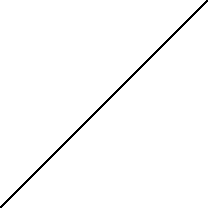
\includegraphics[scale=0.8]{intro-curve} & 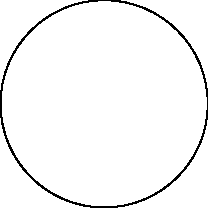
\includegraphics[scale=0.8]{intro-curve3} & 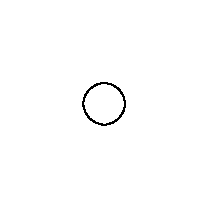
\includegraphics[scale=0.8]{intro-curve2}
		& 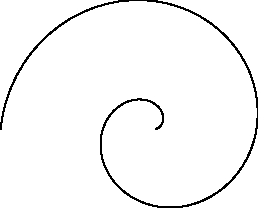
\includegraphics[scale=0.8]{intro-curve4} \\[5pt]
		Zero curvature & Small curvature & Larger curvature
		& Variable curvature
	\end{tabular}
\end{center}

Understanding and quantifying this concept for more complicated curves is our first important goal. The rough idea is to imagine a curve as a roller-coaster along which you travel at a constant speed; the curvature is then the \emph{force} necessary to keep you travelling along the curve.\smallbreak

Curvature is a more difficult concept for surfaces. In particular, we will hunt for quantities which measure how much a surface appears to be dome- or saddle-shaped.
\begin{center}
	\begin{tabular}{c@{\qquad\qquad}c@{\qquad\qquad}c}
		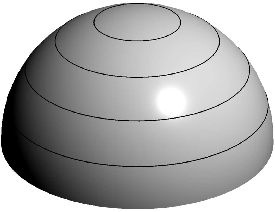
\includegraphics[scale=0.9]{intro-dome} & 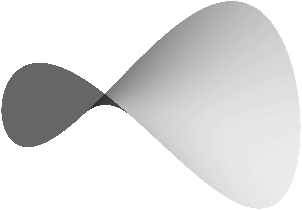
\includegraphics{intro-saddle} & 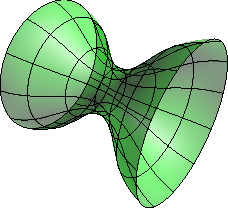
\includegraphics{intro-saddle-dome} \\[5pt]
		Dome-shaped & Saddle-shaped & More complicated
	\end{tabular}
\end{center}
The third surface is saddle-shaped near the narrow neck and dome-shaped away from it.


\section{Curves in Euclidean Space}

\subsection{Euclidean Space, Tangent Vectors \& Regular Curves}\label{sec:euclid}

We begin by refreshing and developing a little notation.

\begin{defn}{}{posvec}
	The set of \emph{$n$-tuples} of real numbers is denoted $\R^n$.\par
	\begin{minipage}[t]{0.7\linewidth}\vspace{-5pt}
		An element can be thought of either as a \emph{point} $P$ or as its \emph{position vector} $\vp=\ray{OP}$ connecting the origin $O=(0,\ldots,0)$ to $P$.\smallbreak
		In co-ordinates, points are typically written as row vectors
		\[P=(\lst{p}{n})\text{ where each }p_i\in\R\]
	\end{minipage}
	\hfill
	\begin{minipage}[t]{0.29\linewidth}\vspace{-15pt}
		\flushright
		\begin{tabular}{c}
			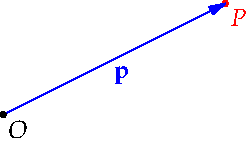
\includegraphics{euclid-posvec}\\
			$\textcolor{red}{P}$ has position vector $\textcolor{blue}{\vp}$
		\end{tabular}
	\end{minipage}\smallbreak
	For vectors, either row or column vector notation is acceptable.\smallbreak
	For each $i$, the \emph{co-ordinate function} $x_i:\R^n\to\R$ returns the $i\th$ co-ordinate of a point: $x_i(P)=p_i$.
\end{defn}


Since the focus of the course is curves and surfaces in 2- and 3-dimensions, we'll mostly restrict to $n\le 3$ and quote theorems in this context.\footnote{For simplicity's sake, we'll almost always state theorems in $\R^3$. The majority are valid in $\R^n$ with a simple notational modification $\{x,y,z\}\rightsquigarrow \{x_1,\ldots,x_n\}$. For $\R^2$ just delete $z=x_3$; many results even make sense in $\R=\R^1$!} We typically use $x,y,z$ for the standard (rectangular) co-ordinate functions
\[
	x(P)=p_1,\quad y(P)=p_2,\quad z(P)=p_3
\]
You should be comfortable with this notation from previous classes and, in particular, with \emph{partial derivatives} of functions defined in terms of the co-ordinate functions $x,y,z$.

\begin{examples}{}{}
	\exstart If $P=(3,1,5)\in\R^3$, then $y(P)=1$.
	\begin{enumerate}\setcounter{enumi}{1}
	  \item The function $f:\R^3\to\R$ defined by $f=x^3\sin(yz)$ has partial derivatives
	  \[
	  	\partials[f]{x}=3x^2\sin(yz)\qquad \partials[f]{y}=x^3z\cos(yz)\qquad \partials[f]{z}=x^3y\cos(yz)
	  \]
	\end{enumerate}
\end{examples}

A \emph{vector} is a directed line segment joining two \emph{points.} We've already seen the \emph{position vector} of a point $P$, namely $\ray{OP}$. In differential geometry it is crucial to distinguish the vectors \emph{based} at a given point.

\begin{defn}[lower separated=false, sidebyside, sidebyside align=top seam, sidebyside gap=0pt, righthand width=0.22\linewidth]{}{tanvec}
	A \emph{tangent vector} $\vv_p$ is a \emph{pair} of elements of $\R^3$: a \emph{\textcolor{blue}{base point}} $p$ and a \emph{\textcolor{red}{direction}} $\vv$.
	It is the directed line segment from the point with position vector $\vp$ to the point with position vector $\vp+\vv$.\medbreak
	The \emph{tangent space at $p$} is the set $T_p\R^3$ of all tangent vectors based at $p$. At each point, $\R^3$ has a \emph{different tangent space}!
	\tcblower
	\flushright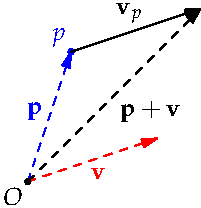
\includegraphics{euclid-tanvec}
\end{defn}

Be aware that $\vv_p=\vw_q\iff p=q$ \emph{and} $\vv=\vw$: the same \emph{direction} at different \emph{base points} means a different tangent vector!
\medbreak

\begin{minipage}[t]{0.6\linewidth}\vspace{0pt}
	The tangent space at $p$ is suitably named, for it is indeed a \emph{vector space}: to add tangent vectors $\vv_p,\vw_p\in T_p\R^3$, simply sum the \emph{direction vectors}
	\[
		\vv_p+\vw_p:=(\vv+\vw)_p\tag{$\ast$}
	\]
	Scalar multiplication is similar: $\lambda\vv_p:=(\lambda\vv)_p$. 
\end{minipage}
\hfill
\begin{minipage}[t]{0.39\linewidth}\vspace{0pt}
	\flushright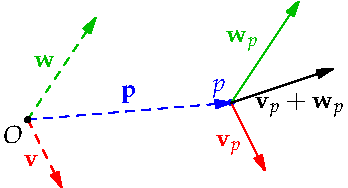
\includegraphics{euclid-tanvec2}
\end{minipage}\medbreak

In chapter \ref{chap:forms} we will see a more abstract discussion of tangent vectors, vector fields, and their application.


\boldsubsubsection{Euclidean Space: $\E^n$ versus $\R^n$}

To describe curves and surfaces in differential geometry, we \emph{parametrize} using functions.

\begin{example}{}{circlebasic}
	There are multiple ways to do this for a given curve: for instance
	\[
		\vx:(-\pi,\pi]\to \R^2: t\mapsto \bigl(\cos t,\sin t\bigr)\quad \text{and} \quad\vy:\R\to\R^2:s\mapsto \left(\frac{1-s^2}{1+s^2},\frac{2s}{1+s^2}\right)
	\]
	both parametrize (most of) the unit circle in the plane ($\vy$ ignores the point $(-1,0)$).
\end{example}

Plainly the \emph{codomain} $\R^2$ is where the geometric action is: in the above we have the same circle, and concepts such as \emph{length} and \emph{angle} can be measured. This extra structure motivates us to distinguish the codomain with new notation.

\begin{defn}{}{dotprod}
	\emph{Euclidean space} $\E^n$ is $\R^n$ equipped with the usual \emph{dot product.} Specifically in $\E^3$:
	\begin{quote}
		The \emph{dot product} of $\vp$ and $\vq$ is $\displaystyle\vp\cdot\vq=\vp^T\vq=(p_1\ p_2\ p_3)\sthreevec{q_1}{q_2}{q_3}=p_1q_1+p_2q_2+p_3q_3$\smallbreak
		The \emph{length} of $\vp$ is $\displaystyle\Nm\vp=\sqrt{\vp\cdot\vp}=\sqrt{p_1^2+p_2^2+p_3^2}$\smallbreak
		The \emph{angle} $\theta$ between $\vp$ and $\vq$ satisfies $\displaystyle\cos\theta=\smash[t]{\frac{\vp\cdot\vq}{\Nm\vp\Nm\vq}}$\smallbreak
		Vectors are \emph{orthogonal}/\emph{perpendicular} if $\vp\cdot\vq=0$, equivalently $\theta=\frac\pi 2$; we write $\vp\perp\vq$.
	\end{quote}
\end{defn}


\boldsubsubsection{Curves in $\E^2$ and $\E^3$}

This course is primarily concerned with \emph{functions} $\vx:U\subseteq\R^m\to\E^n$. In particular:
\begin{description}\itemsep0pt
	\item[\normalfont\emph{Plane curves}:] $m=1$ and $n=2$; for example the above circle.
	\item[\normalfont\emph{Spacecurves}:] $m=1$ and $n=3$; we'll see several momentarily.
	\item[\normalfont\emph{Surfaces}:] $m=2$ and $n=3$. For instance, the parametrization $\vx:\R^2\mapsto\E^3:(u,v)\mapsto (u,v,u^2+v^2)$ of a \emph{paraboloid} should be  familiar.
\end{description}

Surfaces are the focus of Chapter \ref{chap:surfaces}. It is now time for the formal definition of a curve.

\goodbreak
 


\begin{defn}{}{regcurve}
	A \emph{(smooth parametrized) curve} is a function, $\vx:I\to\E^3$, $\vx(t)=\bigl(x(t),y(t),z(t)\bigr)$, defined on an interval $I$ and whose components $x,y,z$ are infinitely differentiable\footnotemark\ everywhere on $I$.\par
	Its \emph{derivative} (also \emph{velocity} or \emph{tangent vector}) is denoted\par
	\begin{minipage}[t]{0.7\linewidth}\vspace{-10pt}
		\[
			\vx'(t)=\diff[\vx]{t}=\bigl(x'(t),y'(t),z'(t)\bigr)
		\]
		The curve's \emph{speed} is the continuous scalar function 
		\[
			v(t)=\Nm{\vx'(t)}=\sqrt{x'(t)^2+y'(t)^2+z'(t)^2}
		\]
		A curve is \emph{regular} if its \emph{tangent vector} $\vx'(t)$ is everywhere non-zero. 
	\end{minipage}
	\hfill
	\begin{minipage}[t]{0.29\linewidth}\vspace{0pt}
		\flushright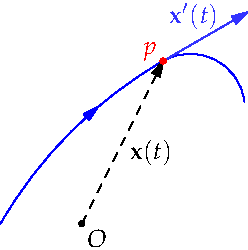
\includegraphics{curves-tangent-vector}
	\end{minipage}
\end{defn}

\footnotetext{The meaning of \emph{smooth} depends on the author: at a minimum it means that  $x,y,z$ must be \emph{differentiable with continuous derivative.} We take the maximal approach for simplicity.}

In the context of Definitions \ref{defn:posvec} and \ref{defn:tanvec}, note that for each $t\in I$:
\begin{quote}
	$\vx(t)$ is a \emph{position vector} whose nose describes the location of a point on the curve.\smallbreak
	$\vx'(t)\in T_p\E^3$ is a \emph{tangent vector} based at the point $p$ with position vector $\vx(t)$.
\end{quote}

A parametrized curve has an \emph{orientation} (indicated by the blue arrow): as $t$ increases along the interval $I$, the point $\vx(t)$ moves in a particular direction along the curve.


\begin{minipage}[t]{0.69\linewidth}\vspace{0pt}
	\begin{examples}{}{}
		\hangindent\leftmargini
		\emph{Straight line}: The line through points with position vectors $\va,\vb$ may be parametrized by
		\[
			\vx(t)=\va+t(\vb-\va)=(1-t)\va+t\vb
		\]
		The tangent vector at $\vx(t)$ is the constant $\vx'(t)=\vb-\va$ and the parametrization has constant speed $\Nm{\vb-\va}$. For instance,
		\[
			\vx(t)=\bigl(2+t,3-2t\bigr)
		\]
		has constant velocity $\vx'(t)=(1,-2)$ and speed $v(t)=\sqrt 5$.
		\begin{description}
		  \item[\normalfont\emph{Circle}] (Example \ref{ex:circlebasic}) The parametrization $\vx(t)=\bigl(\cos t,\sin t\bigr)$ has velocity $\vx'(t)=\bigl(-\sin t,\cos t\bigr)$ and constant speed $v(t)=1$.\par
		  By contrast, $\vy(s)=\tfrac 1{1+s^2}\bigl(1-s^2,2s\bigr)$ has non-constant speed
		  \[
		  	\vy'(s)=\frac 2{(1+s^2)^2}\bigl(-2s,1-s^2\bigr)\qquad v(s)=\frac 2{1+s^2}
		  \]
		  A particle moves quickest at $s=0$ when $v(0)=2$ and the speed tends to zero as $s\to\pm\infty$ (see the linked animation).
		\end{description}
	\end{examples}
\end{minipage}
\hfill
\begin{minipage}[t]{0.3\linewidth}\vspace{0pt}
	\flushright 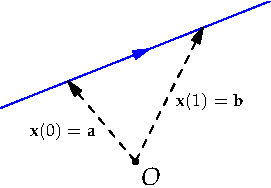
\includegraphics{curves-line}\par
	\flushright	\href{http://www.math.uci.edu/~ndonalds/math162a/curves-animcircle.html}{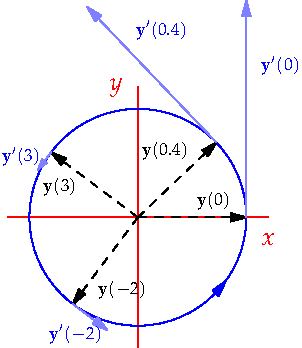
\includegraphics{curves-animcircle2}}
\end{minipage}

\clearpage


\begin{tcolorbox}[exstyle,title={}]
	\begin{description}
		\begin{minipage}[t]{0.72\linewidth}\vspace{0pt}
		  \item[\normalfont\emph{Helix}] $\vx(t)=\bigl(\cos t,\sin t,t\bigr)$ parametrizes a \emph{helix} (ascending spiral).\par
		  To help visualize this, imagine sitting on top of the $z$-axis and looking down; you'd see its horizontal projection $t\mapsto\bigl(\cos t,\sin t\bigr)$ (a counter-clockwise circle). Since $z(t)=t$, the curve moves upwards at constant speed. One can similarly project onto the $xz$- and $yz$-planes.\bigbreak
			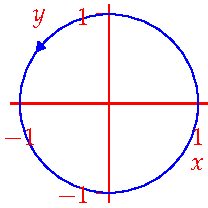
\includegraphics[scale=1]{curves-helix2}\quad
			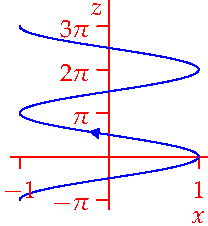
\includegraphics[scale=1]{curves-helix3}\quad
			\makebox[0cm][l]{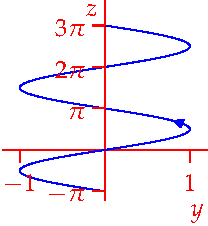
\includegraphics[scale=1]{curves-helix4}}
		\end{minipage}
		\hfill
		\begin{minipage}[t]{0.27\linewidth}\vspace{0pt}
			\flushright	\href{http://www.math.uci.edu/~ndonalds/math162a/curves-helixnew.html}{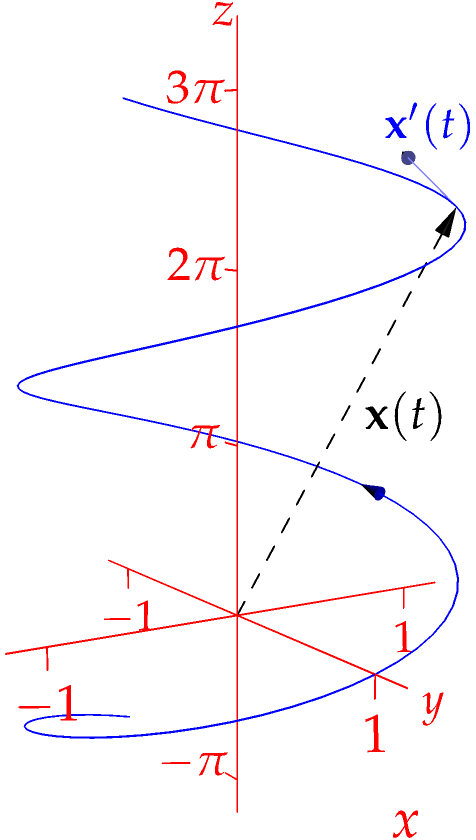
\includegraphics{curves-helixnew}}
		\end{minipage}\par
		The tangent vector at $\vx(t)$ is $\vx'(t)=\bigl(-\sin t,\cos t,1\bigr)$ and the speed is constant $v(t)=\sqrt 2$.
	
		\begin{minipage}[t]{0.72\linewidth}\vspace{0pt}
		  \item[\normalfont\emph{Tangent Line}] Let $\vx:I\to\E^3$ be regular and $t_0\in I$ be fixed. The \emph{tangent line at $\vx(t_0)$} is simply the straight line through the point with position vector $\vx(t_0)$ oriented in the direction of the tangent vector $\vx'(t_0)$. It is itself a parametrized curve, $\vy:\R\to\E^3$:
			\[
				\vy(s)=\vx(t_0)+s\vx'(t_0)
			\]
			For example, the tangent line to the above helix at $t_0=\frac{7\pi}3$ is
			\[
				\vy(s)=\left(\frac 12,\frac{\sqrt 3}2,\frac{7\pi}3\right)+\left(-\frac{\sqrt 3}2,\frac 12,1\right)s
			\]
			The tangent line has the same speed as the helix $\sqrt 2$.
		\end{minipage}
		\hfill
		\begin{minipage}[t]{0.27\linewidth}\vspace{0pt}
			\flushright	\href{http://www.math.uci.edu/~ndonalds/math162a/curves-helixnewtan.html}{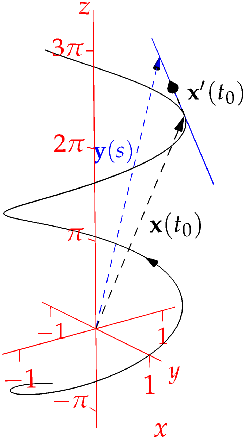
\includegraphics[scale=0.95]{curves-helixnewtan}}
		\end{minipage}\par
	
	
		\begin{minipage}[t]{0.68\linewidth}\vspace{-10pt}
			\item[\normalfont\emph{Self-intersections}] These are no problem for our formulation!	The curve
			\[
				\vx(t)=\left(\sin\tfrac{2t}3,\cos t\right),\quad t\in [0,6\pi)
			\]
		 	passes through the origin at both $t_1=\frac{3\pi}2$ and $t_2=\frac{9\pi}2$, with corresponding tangent vectors
			\[
				\textcolor{blue}{\vx'(\tfrac{3\pi}2)}=\left(-\tfrac 23,1\right),\qquad \textcolor{Green}{\vx'(\tfrac{9\pi}2)}=\left(-\tfrac 23,-1\right)
			\]
			In this example, we shouldn't talk about \emph{the} tangent vector to the curve \emph{at the origin,} since it is non-unique. Rather we should refer to the \emph{co-ordinates} $\frac{3\pi}2$ or $\frac{9\pi}2$.
		\end{minipage}
		\hfill
		\begin{minipage}[t]{0.31\linewidth}\vspace{0pt}
			\flushright	\href{http://www.math.uci.edu/~ndonalds/math162a/curves-selfint.html}{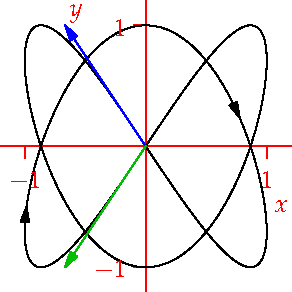
\includegraphics[scale=0.95]{curves-selfint}}
		\end{minipage}\par
		The linked animation shows the variable speed $v(t)=\sqrt{\frac{4}{9}\cos^2\frac{2t}{3}+\sin^2t}$ of this curve.
	\end{description}
\end{tcolorbox}

\goodbreak

\boldinline{Corners and Cusps} To ensure that a tangent direction exists, a regular curve has everywhere non-zero derivative. Here are a couple of examples of curves with non-regular points.

\begin{examples}[lower separated=false, sidebyside, sidebyside align=top seam, sidebyside gap=0pt, righthand width=0.34\linewidth]{}{}
	\hangindent\leftmargini
	\emph{Corner}\lstsp A curve might enter and leave a point in different directions. For example, $\vx(t)=\bigl(t,1-\nm t\bigr)$ has derivative
	\[\vx'(t)=\begin{cases}
	(1,1)&\text{if }t<0\\
	(1,-1)&\text{if }t>0
	\end{cases}\]
	At $\vx(0)=(0,1)$ the curve is non-differentiable and thus non-smooth and non-regular.
	\begin{description}
		\item[\normalfont\emph{Cusp}] The curve $\vx(t)=\bigl(t^3,t^2\bigr)$ has derivative 	\[\vx'(t)= \left(3t^2,2t\right)\]
		The origin is a \emph{cusp,} a special type of corner where the curve leaves the point in the opposite direction to how it entered. In this case the curve is differentiable at the origin, but is non-regular since its speed $v(0)$ is zero.
	\end{description}
	\tcblower
	\flushright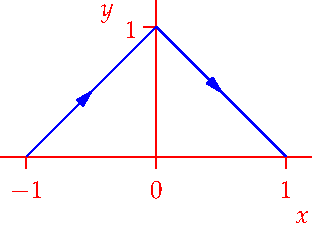
\includegraphics{curves-corner}\\
	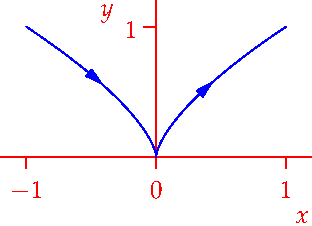
\includegraphics{curves-cusp}
\end{examples}

\vfil

\begin{exercises}
	\exstart A twice-differentiable curve $\vx(t)$ has the property that its second derivative $\vx''(t)$ is identically zero. What can be said about $\vx$?
	\begin{enumerate}\setcounter{enumi}{1}  
		\item Find the unique curve such that $\vx(0)=(1,0,5)$ and $\vx'(t)=(t^2,t,e^t)$.
		
		\item An ellipse in the plane has equation $\frac{x^2}4+\frac{y^2}9=1$. By modifying the standard parametrization of the circle, find a regular parametrization of this ellipse. What is its speed?
		
		\item Show that $\vx(t)=\bigl(\frac{e^t+e^{-t}}2,\frac{e^{t}-e^{-t}}2)$ parametrizes half of the hyperbola $x^2-y^2=1$. How would you parametrize the other half?
		
	  \item\label{exs:regnonintrinsic}\begin{enumerate}
	    \item Find the speed of the re-parametrized standard helix $\vy(s)=\vx(s^3)=\bigl(\cos s^3,\sin s^3,s^3\bigr)$.
	    \item More generally, if $\vx(t)$ is a regular curve, show that $\vy(s):=\vx(s^3)$ is non-regular. 
	  \end{enumerate}
	  
		\item Verify that our cusp example (above) may instead be parametrized $\vy(u)=\bigl(u,u^{2/3}\bigr)$. Is the new parametrization still non-regular at the origin? Explain.
		
		\item Show that the tangent vectors to the regular curve $\vx(t)=\bigl(3t,3t^2,2t^3\bigr)$ make a constant angle with the vector $(1,0,1)$.
		
		\item Consider the plane curve $\vx(t)=\bigl(t-1+e^{-t}, e^{-t}\bigr)$. Find the equation of its tangent line at $t=t_0$ and find where the tangent line intersects the $x$-axis.
	
		\item\label{exs:graphparam} Let $f:\R\to\R$ be a smooth function. Find a parametrization for the graph of $y=f(x)$ and find its tangent line when $x=x_0$.
	
		\item Find a parametrization of the straight line through the points $(1,-3,-1)$ and $(6,2,1)$. Does this line meet the line through the points $(-1,1,0)$ and $(-5,-1,-1)$?
	\end{enumerate}
\end{exercises}

\clearpage


\subsection{The Arc-length Parametrization and Curvature}\label{sec:arclength}

As we've seen, the same `curve' (viewed as a subset of $\E^3$) may be parametrized in different ways. For instance, in Exercise \ref*{sec:euclid}.\ref{exs:regnonintrinsic}, the standard helix $\vx(t)=(\cos t,\sin t,t)$ was re-parametrized to obtain
\[
	\vy(s)=(\cos s^3,\sin s^3,s^3)\tag{$\ast$}
\]
This new parametrization is non-regular at $s=0$; it \emph{slows down and stops} before resuming its journey up the helix! Regularity is not, therefore, an intrinsic property of a curve viewed as a \emph{set} ($\operatorname{range}(\vx)$), rather it is a property of the parametrization.\smallbreak

Thankfully it is easy to create new parametrizations that remain regular.

\begin{lemm}{}{reparam}
	If $\vx:I\to\E^3$ is regular and $\alpha:J\to I$ is smooth with nowhere-zero derivative, then we obtain a new \emph{regular} parametrization
	\[
		\vy:J\to\E^3,\quad \vy(s):=\vx\bigl(\alpha(s)\bigr)
	\]
\end{lemm}

\begin{proof}\def\range{\operatorname{range}}
	By the chain rule, $\diff[\vy]{s}=\alpha'(s)\diff[\vx]{t}$, which is non-zero by assumption.
\end{proof}

By contrast, if $\vx(t)$ is non-regular, no smooth reparametrization can possible regularize it.\medbreak


Since $\alpha'(s)$ is continuous and non-zero, there are two distinct cases:\footnote{Observe that $\alpha'(s)$ is \emph{always positive} or \emph{always negative.} In particular, $\alpha(s)$ is 1--1. If, in addition, $\alpha$ is \emph{onto,} then $\vx$ and $\vy$ parametrize precisely the same subset of $\E^3$.}
\begin{description}
	\item[\normalfont\emph{$\alpha(s)$ increasing}] We call this an \emph{orientation-preserving} re-parametrization, since a `particle' travels along the curve in the same direction.
	\item[\normalfont\emph{$\alpha(s)$ decreasing}] The re-parametrization is \emph{orientation-reversing.}
\end{description}

In the language of the Lemma, ($\ast$) turned a regular parametrization into a non-regular one because $\alpha(s)=s^3$ has $\alpha'(s)=3s^2$ which is zero at $s=0$.\bigbreak

Our next goal is to develop a special parametrization for regular curves. First we recall a concept from multi-variable calculus.

\begin{defn}{}{}
	The (signed) \emph{arc-length} of a curve $\vx:I\to\E^3$ measured from $\vx(t_0)$ to $\vx(t)$ is the integral of the speed
	\[
		s(t)=\int_{t_0}^t\Nm{\vx'(T)}\D T =\int_{t_0}^tv(T)\,\D T
	\]
\end{defn}

The arc-length is \emph{signed} because it is negative if $t<t_0$: we are measuring length against the orientation of the curve. Of course if $\vx:[a,b]\to\E^3$ has domain a closed bounded interval, then it is most sensible to measure arc-length from $t_0=a$ so that $s(t)\ge 0$ everywhere on the curve.

\begin{example}{}{}
	The standard helix $\vx(t)=\bigl(\cos t,\sin t,t\bigr)$ has constant speed $\sqrt 2$, whence the arc-length measured from $\vx(0)$ is simply $s(t)=\sqrt 2t$.
\end{example}

Recall the Fundamental Theorem of Calculus: is $s(t)$ is the arc-length of a regular curve, then
\[
	\diff[s]{t}=\diff t\int_{t_0}^t\Nm{\vx'(T)}\,\D T=\Nm{\vx'(t)}=v(t)
\]
is the curve's speed, which is \emph{positive} and \emph{continuous.} The same is therefore true for its \emph{inverse function}
\[
	\diff[t]{s}=\frac 1{s'(t)}=\frac 1{v(t)}>0
\]

\begin{defn}{}{}
	An \emph{arc-length parameter} for a regular curve $\vx(t)$ is the inverse $\alpha(s)=t(s)$ of an arc-length function $s(t)$.
\end{defn}

Lemma \ref{lemm:reparam} tells us that $\vy(s)=\vx\bigl(\alpha(s)\bigr)$ is a regular re-parametrization of our original curve. Indeed it is a re-parametrization with a very special property:
\[
	\Nm{\vy'(s)}=\alpha'(s)\Nm{\vx'\bigl(\alpha(s)\bigr)}=\frac 1{v(t)}v(t)=1 \tag{$\dag$}
\]
The curve $\vy(s)$ has \emph{unit-speed.} We have therefore proved a key result.

\begin{thm}{}{unitspeed}
	Every regular curve has a unit-speed parametrization, namely by an arc-length parameter  (measured from wherever you like).
\end{thm}

The usefulness of the Theorem is abstract; by \emph{assuming} that we have a unit-speed parametrization, certain analyses become much simpler. As a practical matter, explicitly finding an arc-length parametrization might be essentially impossible (evaluate an integral then invert a function\ldots).

\begin{examples}{}{}
	\exstart Since the standard helix has arc-length parameter $s(t)=\sqrt 2t$, it is trivial to observe that the re-parametrization
	\[
		\vy(s)=\left(\cos\frac s{\sqrt 2},\sin\frac s{\sqrt 2},\frac s{\sqrt 2}\right)
	\]
	has unit speed.
	\begin{enumerate}\setcounter{enumi}{1}
	  \item More generally, if $\vx(t)$ has constant speed $v$, then $s(t)=vt$ is an arc-length parameter and $\vy(s)=\vx(\tfrac sv)$ a unit-speed re-parametrization.
	  \item The graph of $y=\frac 23x^{3/2}$ ($t\ge 0$) may be parametrized by $\vx(t)=(t,\frac 23t^{3/2})$. The arc-length measured from the origin is then
	  \[
	  	s(t)=\int_0^t\sqrt{1+T}\,\D T =\tfrac 23\left[(1+t)^{3/2}-1\right] \implies \alpha(s)=t(s)=\left(1+\tfrac 32s\right)^{2/3}-1
	  \]
	  We've obtained an explicit unit-speed parametrization
	  \[
	  	\vy(s)=\vx\bigl(\alpha(s)\bigr) =\left(\left(1+\tfrac 32s\right)^{2/3}-1,\tfrac 23\left[\left(1+\tfrac 32s\right)^{2/3}-1\right]^{3/2}\right)
	  \]
	  though is it really something you ever want to compute with?!
	%   \item
	%   \[s(t)=\int_0^t\sqrt{1+4T^2}\,\D T\]
	%   This can be computed with some judicious use of substitutions,\footnote{Try $\tan\theta=2T\ldots$} though it isn't fun!
	%   \[s(t)=\frac 12t\sqrt{1+4t^2}+\frac 14\ln\nm{2t+\sqrt{1+4t^2}}\]
	%   Now you need an inverse! This problem is essentially impossible to do explicitly.
	%   \item At least where it is regular, $\vx(t)=\twovec{t}{1-\nm t}$ has speed $v(t)=\sqrt{2}$ ($t\neq 0$). Thus $\vx(s)=\twovec{s/\sqrt{2}}{1-\nm{s/\sqrt{2}}}$ is a unit speed parametrization, away from $s=0$.
	%   \item Explicitly finding a unit speed parametrization of $\vx(t)=\twovec{\sin\frac{2t}{3}}{\cos t}$ is also far too difficult. It would involve computing the integral
	%   \[s(t)=\int_0^t\sqrt{\frac 49\cos^2\frac{2T}3+\sin^2T}\D T\] 
	
		\goodbreak
		
	% 	\item\label{ex:catenary1} A \emph{catenary} is famously the shape made by a rope/chain hanging between two fixed points. In suitable co-ordinates it has equation\footnotemark\ $y=\cosh x=\frac{e^x+e^{-x}}2$. As a parametrized curve
	% 	\[\vx(t)=\bigl(t,\cosh t\bigr)\implies \vx'(t)=\bigl(1,\sinh t\bigr)\implies v(t)=\sqrt{1+\sinh^2t}=\cosh t\]
	% 	\begin{minipage}[t]{0.6\linewidth}\vspace{-3pt}
	% 		The arc-length measured from $t_0=0$ is
	% 		\[s(t)=\int_0^t\cosh T\,\D T=\sinh t\tag{$\dag$}\]
	% 		from which
	% 		\[\vy(s)=\vx\bigl(\sinh^{-1}s\bigr)=\bigl(\sinh^{-1}s,\sqrt{1+s^2}\bigr)\]
	% 		has unit speed, as can be checked explicitly:
	% 		\[\makebox[0cm][l]{$\displaystyle\vy'(s)=\frac{1}{\sqrt{1+s^2}}\bigl(1,s\bigr) \implies\Nm{\vy'(s)}^2=\frac{1}{1+s^2}+\frac{s^2}{1+s^2}=1$}\]    
	% 	\end{minipage}\hfill\begin{minipage}[t]{0.4\linewidth}\vspace{-8pt}
	% 		\flushright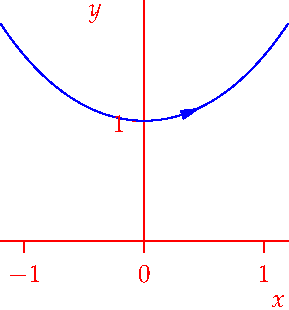
\includegraphics{regular-catenary}
	% 	\end{minipage}
	\end{enumerate}
\end{examples}

% \footnotetext{If the hyperbolic functions are unfamiliar, you can do the example purely with exponentials and logarithms. All we really need is the following:
% \[\cosh x=\frac{e^x+e^{-x}}2,\quad \sinh x=\frac{e^x-e^{-x}}2 \implies \diff x\cosh x=\sinh x,\quad \diff x\sinh x=\cosh x,\quad \cosh^2\!x-\sinh^2\!x=1\]
 %To invert $(\dag)$, you need to solve a quadratic in $e^t$:
%\[s=\frac{e^t-e^{-t}}2\implies (e^t)^2-2se^t-1=0\implies t=\sinh^{-1}s=\ln(s+\sqrt{1+s^2})\]
%}

\medskip


Armed with unit-speed curves, we can now define our principal notion of bendiness.

\begin{defn}{}{curvature}
	The \emph{curvature} of a unit-speed curve $\vx:I\to\E^3$ is 
	\[
		\kappa(s)=\Nm{\vx''(s)}
	\]
	We modify this slightly for curves in the plane: $\kappa(s)$ is positive/negative if the tangent vector rotates \emph{counter-clockwise}/\emph{clockwise} as we traverse the curve. This corresponds to the usual \emph{right hand rule.}
\end{defn}

By Newton's second law, a unit mass travelling along the curve at unit speed experiences a \emph{transverse force} of magnitude $\kappa(s)$.

\begin{examples}{}{}
	\exstart A straight line has curvature zero. For example, the line joining $(1,4)$ and $(-3,1)$ has unit-speed parametrization $\vx(s)=\bigl(-3+\frac 45s,1+\frac 35s\bigr)$, whence $\vx''(s)=\V0\implies \kappa(s)=0$.

	\begin{enumerate}\setcounter{enumi}{1}
	  \item The circle of radius $r$ has unit-speed parametrization $\vx(s)=r\left(\cos\frac sr,\sin\frac sr\right)$, whence
	  \[
	  	\vx''(s)=-\frac 1r\twovec{\cos\frac sr}{\sin\frac sr}\implies \kappa(s)=\frac 1r
	  \]
	  This is positive since the tangent vector rotates counter-clockwise. Observe that $\kappa=\frac 1r$ is inversely proportional to the radius: smaller circles have larger curvature.
	    
	  \item The standard helix with unit-speed parametrization $\vx(s)=\smash[b]{\left(\cos\frac s{\sqrt 2},\sin\frac s{\sqrt 2},\frac s{\sqrt 2}\right)}$ has
	  \[
	  	\vx''(s)=-\frac 12\left(\cos\frac s{\sqrt 2},\sin\frac s{\sqrt 2},0\right)\implies \kappa(s)=\frac 12
	  \]
	  
	%   \item The above catenary has
	%   \[\vy''(s)=\frac 1{(1+s^2)^{3/2}}\bigl(-s,1\bigr)\implies \kappa(s)=\frac 1{1+s^2}\]
	%   The picture convinces us that this should be positive. Moreover, $\vy(0)$ is the point of maximum curvature $\kappa=1$ at the bottom of the curve. As we move away, the curvature decreases and the curve becomes straighter.
	\end{enumerate}
\end{examples}

Since finding a unit-speed parametrization is difficult, there few curves for which this approach is sensible. What we want is a method that works for \emph{arbitrary parametrization.} This is indeed possible, though for spacecurves it will take a while. For curves in the \emph{plane} however, things are fairly easy.


\boldinline{Curvature of Plane Curves}

If $\vy:I\to\E^2$ has unit-speed, we can write\par
\begin{minipage}[t]{0.72\linewidth}\vspace{-12pt}
	\[
		\vy'(s)=\textcolor{blue}{\twovec{\cos\theta(s)}{\sin\theta(s)}}
	\]
	where $\theta(s)$ is the \emph{angle} between the tangent line and the positive $x$-axis. Now observe that
	\[
		\vy''(s)=\theta'(s)\textcolor{Green}{\twovec{-\sin\theta(s)}{\cos\theta(s)}}
	\]
	Since $\bigl(-\sin\theta,\cos\theta\bigr)$ points to the \emph{left} of $\vy'(s)$, we conclude:
\end{minipage}
\hfill
\begin{minipage}[t]{0.27\linewidth}\vspace{-8pt}
	\flushright 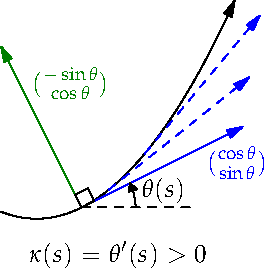
\includegraphics[scale=0.95]{regular-planekappa}
\end{minipage}\par


\begin{thm}{}{kappaplane}
	The curvature of a unit-speed plane curve is the rate of change $\kappa(s)=\theta'(s)$ of the angle of its tangent line.
\end{thm}

This should be intuitive for constant curvature examples such as the straight line and the circle.

\goodbreak

Now suppose $\vx(t)=\bigl(x(t),y(t)\bigr)$ is any regular parametrization of the same curve; its speed satisfies
\[
	v(t)=\sqrt{x'(t)^2+y'(t)^2}=s'(t)
\]
where $s(t)$ is an arc-length function for $\vx(t)$. Moreover, the angle $\theta(s)$ plainly satisfies
\[
	\theta(s)=\tan^{-1}\frac{y'(t)}{x'(t)}
\]
Now differentiate and applying the chain rule:
\[
	\kappa(s)=\diff s\tan^{-1}\frac{y'(t)}{x'(t)} =\diff[t]{s}\diff t\tan^{-1}\frac{y'(t)}{x'(t)} =\cdots
\]
% \left(\frac 1{s'(t)}\right)\frac{y''x'-x''y'}{(x')^2\left[1+\left(\frac{y'}{x'}\right)^2\right]}\]
The result is a formula for the curvature as a function of an arbitrary regular parametrization.

\begin{cor}{}{kappagraph}
	A regular curve $\vx(t)=\bigl(x(t),y(t)\bigr)$ has curvature
	\[
		\kappa(t)=\frac{y''x'-x''y'}{[x'^2+y'^2]^{3/2}} =\frac{y''x'-x''y'}{v^3} =\frac{\vx''\cdot J\vx'}{v^3}
	\]
	where $J\vx'=\scalebox{0.75}{$\begin{pmatrix}
	0&-1\\1&0
	\end{pmatrix}$}\stwovec{x'}{y'}=\stwovec{-y'}{x'}$. In particular, the graph of a smooth function $y=f(x)$ has curvature
	\[
		\kappa(x)=\frac{f''(x)}{\Bigl[1+\bigl(f'(x)\bigr)^2\Bigr]^{3/2}}
	\]
\end{cor}


\begin{examples}{}{}
	\exstart The graph of $y=\frac 23x^{3/2}$ has curvature
	\[
		\kappa(x)=\frac{\frac 12x^{-1/2}}{(1+x)^{3/2}}= \frac 1{2\sqrt{x(1+x)^3}}
	\]
	\begin{enumerate}\setcounter{enumi}{1}
	  \item If $f(x)=\sin x$, then $\kappa(x)=\dfrac{-\sin x}{(1+\cos^2\!x)^{3/2}}$
	  \item The spiral $\vx(t)=\bigl(t\cos t,t\sin t\bigr)$ has
	  \begin{align*}
		  \vx'(t)&=\twovec{\cos t-t\sin t}{\sin t+t\cos t},\quad \vx''(t)=\twovec{-2\sin t-t\cos t}{2\cos t-t\sin t}\\
		  \implies \kappa(t)&=\frac{(2\cos t-t\sin t)(\cos t-t\sin t)-(-2\sin t-t\cos t)(\sin t+t\cos t)}{\left[(\cos t-t\sin t)^2+(\sin t+t\cos t)^2\right]^{3/2}}\\
		  &=\frac{2+t^2}{\left[1+t^2\right]^{3/2}}
	  \end{align*}
	\end{enumerate}
\end{examples}


\clearpage

\begin{exercises}
	\exstart Compute the arc-length of the following curves by parametrizing and evaluating an integral:\vspace{-5pt}
	
	\begin{enumerate}\setcounter{enumi}{1}
	  \item[]\begin{enumerate}
	    \item The straight line between points $(3,1,2)$ and $(1,1,0)$.
	    \item The circle centered at $(1,-2)$ with radius 5 measured \emph{clockwise} from $(6,-2)$ to $(1,3)$.
	    \item The graph of the function $y=\frac 23x^{3/2}-\frac 12x^{1/2}$ for $1\le x\le 9$.
	  \end{enumerate}
	  
	  \item Find the curvature of the following plane curves (use Corollary \ref{cor:kappagraph}).
	  \begin{enumerate}
	    \item The graph of $y=x^2$.
	    \item The catenary: the graph of $y=\frac 12(e^x+e^{-x})=\cosh x$
	    \item The figure-eight curve $\vx(t)=\bigl(\cos t,\sin 2t\bigr)$
	    \item\label{exs:expspiral} The exponential spiral $\vx(t)=\bigl(e^t\cos t,e^t\sin t\bigr)$.
	  \end{enumerate}
	  
	  \item Find a unit-speed parametrization of the straight line between points with position vectors $\va\neq \vb$ in $\E^3$ and hence verify that its curvature is zero.
	  	
		\item Suppose $\vx:\R\to\E^3$ has unit speed. Verify that $\vx$ is parametrized by an arc-length parameter.
	
	  \item Find the curvature of the spacecurve $\vx(s)=\left(\frac 5{13}\cos s,\sin s,\frac{12}{13}\cos s\right)$. What is this curve?
	  
	  \item\begin{enumerate}
			\item Find the arc-length of the standard helix $\vx(t)=\left(\cos t,\sin t,t\right)$ between $t=-\pi$ and $t=2\pi$.
			\item Suppose a particle travels \emph{down} the standard helix so that $\vy(0)=(1,0,2\pi)$ and such that its speed is $v(t)=2\sqrt{2}t$. Find a parametrization which describes this motion.
			\item Let $r,h$ be positive constants. Find the curvature of the general circular helix
			\[
				\vx(t)=\bigl(r\cos t,r\sin t,ht\bigr)
			\]
			and interpret how it depends on $r$ and $h$.
	\end{enumerate}
	
		\item Check the evaluation of $\kappa(t)$ and $\kappa(x)$ in the proof of Corollary \ref{cor:kappagraph}.
	
	  \item We find the curvature of the exponential spiral $\vx(t)=\bigl(e^t\cos t,e^t\sin t\bigr)$ the hard way.
	  \begin{enumerate}
	    \item Calculate the arc-length $s(t)$ measured from $\vx(0)$.
	    \item Find a unit-speed parametrization $\vy(s)$ where $\vy(0)=(1,0)$.
	    \item Hence compute $\kappa(s)$ and show that it equals your answer from Exercise \ref{exs:expspiral}.%=\frac 1{s+\sqrt 2}$.
	  \end{enumerate}
	
	
		\begin{minipage}[t]{0.5\linewidth}\vspace{0pt}
			\item A circle of radius 1 rolls at constant speed without slipping along the $x$-axis so that the angle indicated in the picture is $t$ at time $t$.\smallbreak
			The \textcolor{blue}{curve} described by a \textcolor{red}{point} on the circumference of the rolling circle is a \emph{cycloid}.
		\end{minipage}
		\hfill
		\begin{minipage}[t]{0.49\linewidth}\vspace{0pt}
			\flushright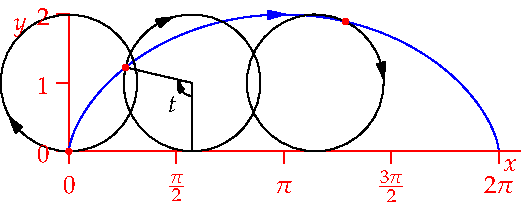
\includegraphics[scale=0.85]{regular-cycloid}
		\end{minipage}\vspace{-15pt}
	
		\begin{enumerate}
			\item Find a parametrization $\vx:[0,2\pi]\to\E^2$.
			\item Find the curvature of the cycloid as a function of $t$.
			\item Compute the arc-length of the cycloid over a complete rotation of the circle.
		\end{enumerate}
		
	\end{enumerate}
\end{exercises}


\clearpage



\subsection{Orthogonality, Moving Frames \& The Structure Equations}\label{sec:orth}

Our plan is to analyze a curve with respect to a family of \emph{moving} orthonormal bases. Before embarking on this, we summarize the relevant ideas from linear algebra. Hopefully most of the concepts are familiar. Most proofs are omitted, but will be met in a standard linear algebra class. As usual, definitions and results are stated in 3-dimensions, but are valid in others, particularly 2-dimensions.\medbreak

In $\E^3$, points are typically denoted with reference to the \emph{standard basis} $\{\vi,\vj,\vk\}$. For instance,
\[
	\vv=\threevec 346=3\vi+4\vj+6\vk
\]
The numbers $3,4,6$ are the \emph{co-ordinates} of $\vv$ with respect to the standard basis. Of course other bases are available\ldots

\begin{defn}{}{}
	A set $\beta=\{\ve_1,\ve_2,\ve_3\}\subseteq\E^3$ is a \emph{basis} if every vector $\vv\in\E^3$ can be expressed uniquely\footnotemark\ as a linear combination of $\ve_1,\ve_2,\ve_3$: that is
	\[
		\vv=c_1\ve_1+c_2\ve_2+c_3\ve_3\tag{$\ast$}
	\]
	for unique $c_1,c_2,c_3\in\R$, the \emph{co-ordinates} of $\vv$ with respect to $\beta$.\smallbreak
	A basis is \emph{orthonormal} if $\ve_j\cdot\ve_k=\delta_{jk}=
	\begin{cases}
		1&\text{if }j=k\\
		0&\text{if }j\neq k
	\end{cases}
	$\smallbreak
	Consider the (invertible) matrix $E=(\ve_1\ \ve_2\ \ve_3)$ whose columns are the elements of $\beta$ viewed as column vectors (with respect to the standard basis). A basis is \emph{positively oriented} if $\det E>0$.
\end{defn}

\footnotetext{In a linear algebra class this is usually broken into two definitions which imply, respectively, the existence and uniqueness of the linear combination $(\ast)$.
\begin{description}
	\item[\normalfont\emph{Spanning Set}] Every $\vv\in\E^3$ can be expressed as a linear combination $\vv=c_1\ve_1+c_2\ve_2+c_3\ve_3$ for some $c_1,c_2,c_3\in\R$.
	\item[\normalfont\emph{Linear Independence}] The only linear combination summing to $\V0$ is trivial: $c_1\ve_1+c_2\ve_2+c_3\ve_3=\V0\implies c_1=c_2=c_3=0$.
\end{description}
}


\begin{examples}{}{basiseasy}
	\exstart $\left\{\frac 1{\sqrt 2}\sthreevec 110,\frac 1{\sqrt 6}\sthreevec 1{-1}{-2},\frac 1{\sqrt 3}\sthreevec 1{-1}1\right\}$ is a \emph{negatively} oriented orthonormal basis of $\E^3$ ($\det E=-1<0$).\par
	\begin{minipage}[t]{0.7\linewidth}\vspace{0pt}
	\begin{enumerate}\setcounter{enumi}{1}
	  \item Every orthonormal basis of $\E^2$ has the form
	  \[
	  	\left\{\textcolor{blue}{\twovec{\cos\theta}{\sin\theta}},\textcolor{Green}{\twovec{-\sin\theta}{\cos\theta}}\right\} \quad\text{or}\quad \left\{\textcolor{blue}{\twovec{\cos\theta}{\sin\theta}},\textcolor{red}{\twovec{\sin\theta}{-\cos\theta}}\right\}
	  \]
	  for some angle $\theta$. The first is positively oriented ($\det=1>0$) and the second negatively ($\det =-1<0$).
	\end{enumerate}
	\end{minipage}\hfill\begin{minipage}[t]{0.29\linewidth}\vspace{0pt}
		\flushright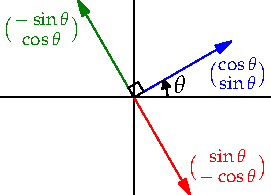
\includegraphics{moving-orthe2}
	\end{minipage}
\end{examples}

A positively oriented orthonormal basis in $\E^3$ satisfies the \emph{right-hand rule}: $\ve_3=\ve_1\times\ve_2$. In $\E^2$, positive orientation means that $\ve_2$ is obtained by rotating $\ve_1$ counter-clockwise by \ang{90}: we can write this as
\[
	\ve_2=J\ve_1=
	\begin{pmatrix}
		0&-1\\1&0
	\end{pmatrix}
	\ve_1
\]

Finding the co-ordinates of a vector with respect to a basis ($\ast$) is really a matrix problem\footnote{For obvious reasons, this is known as the \emph{change of co-ordinate matrix} from $\beta$ to the standard basis $\{\vi,\vj,\vk\}$.}
\[
	\vv=E\threevec{c_1}{c_2}{c_3} \implies \threevec{c_1}{c_2}{c_3} =E^{-1}\vv
\]
Inverting a $3\times 3$ matrix is tedious. Thankfully the co-ordinates can be found more easily if the basis is \emph{orthonormal} just by taking dot products!
\[
	\vv\cdot\ve_i =(c_1\ve_1+c_2\ve_2+c_3\ve_3)\cdot \ve_i =c_i
\]

\begin{lemm}{}{orthcomp}
	If $\beta=\{\ve_1,\ve_2,\ve_3\}$ is an orthonormal basis, then for any vector $\vv\in\E^3$,
	\[
		\vv=(\vv\cdot\ve_1)\ve_1+(\vv\cdot\ve_2)\ve_2+(\vv\cdot\ve_3)\ve_3
	\]
\end{lemm}

\begin{example}{}{}
	$\beta =\{\ve_1,\ve_2\} =\left\{\frac 15\stwovec 43, \frac 15\stwovec{-3}4\right\}$ is a positively oriented orthonormal basis of $\E^2$. With respect to $\beta$, the vector $\vv=\stwovec 11$ can be written
	\[
		\twovec 11=(\vv\cdot\ve_1)\ve_1 +(\vv\cdot\ve_2)\ve_2 =\frac 75\ve_1+\frac 15\ve_2
	\]
\end{example}


\boldinline{Orthogonal Matrices}

Recall Definition \ref{defn:dotprod}. Given $\beta=\{\ve_1,\ve_2,\ve_3\}$ and its associated matrix $E=(\ve_1\ \ve_2\ \ve_3)$, observe that
\[
	E^TE=
	\begin{pmatrix}
		\ve_1^T\\
		\ve_2^T\\
		\ve_3^T
	\end{pmatrix}
	(\ve_1\ \ve_2\ \ve_3)
	=
	\begin{pmatrix}
		\Nm{\ve_1}^2&\ve_1\cdot\ve_2&\ve_1\cdot \ve_3\\
		\ve_2\cdot\ve_1&\Nm{\ve_2}^2&\ve_2\cdot \ve_3\\
		\ve_3\cdot\ve_1&\ve_3\cdot \ve_2&\Nm{\ve_3}^2
	\end{pmatrix}
\]

When $\beta$ is an orthonormal basis, this matrix is very simple.

\begin{defn}{}{}
	A $3\times 3$ matrix $A$ is \emph{orthogonal} if $A^TA=I$ (equivalently $AA^T=I$). The set of all such is denoted $\rO_3(\R)$. In addition, if $\det A=1$, we write $A\in \rSO_3(\R)$ (\emph{special orthogonal matrices}).
\end{defn}

\begin{lemm}{}{orth}
	\exstart If $A\in\rO_3(\R)$, then it is invertible with inverse $A^T$ (also orthogonal).
	\begin{enumerate}\setcounter{enumi}{1}
	  \item The product of two orthogonal matrices is orthogonal.
	  \item\label{lemm:orth3} $A$ is orthogonal if and only if $(A\vx)\cdot (A\vy)=\vx\cdot\vy$ for all vectors $\vx,\vy\in\E^3$.
	  \item Let $\beta=\{\ve_1,\ve_2,\ve_3\}$ and $E=(\ve_1\ \ve_2\ \ve_3)\in M_3(\R)$:
	  \begin{enumerate}
	    \item $E\in\rO_3(\R)\iff \beta$ is an orthonormal basis.
	    \item $E\in\rSO_3(\R)\iff \beta$ is a positively oriented orthonormal basis.
	  \end{enumerate}
	\end{enumerate}
\end{lemm}

Parts 1 and 2 together say that $\rO_3(\R)$ forms a \emph{group} under matrix multiplication; it is therefore known as the \emph{orthogonal group.}\footnote{Knowledge of group theory is not necessary for these notes. \emph{Lie Groups,} of which $\rO_3(\R)$ is an example, are critical to more advanced differential geometry.}

\begin{examples*}{\ref{ex:basiseasy} cont}{}
	\exstart It is no fun to check $E^TE=I$ directly, but since we have an orthonormal basis, the lemma tells us that
	\[
		E=
		\begin{pmatrix}
			\frac 1{\sqrt 2} & \frac 1{\sqrt 6} & \frac 1{\sqrt 3}\\
			\frac 1{\sqrt 2} & \frac{-1}{\sqrt 6} & \frac{-1}{\sqrt 3}\\
			0 & \frac{-2}{\sqrt 6} & \frac 1{\sqrt 3}
		\end{pmatrix}
		\in\rO_3(\R)
	\]
	\begin{enumerate}\setcounter{enumi}{1}
	\item Every $2\times 2$ orthogonal matrix has one of two forms:\par
		\begin{tabular}{@{}p{0.48\linewidth}@{\hspace{0.04\linewidth}}p{0.48\linewidth}@{}}
			\emph{Rotations}\ \ $A_\theta=
			\scalebox{0.8}{
				$\begin{pmatrix}
	  			\cos\theta&-\sin\theta\\
	  			\sin\theta&\cos\theta
				\end{pmatrix}$
			}
			\in \rSO_2(\R)$\smallbreak
	  	The effect of the map $\vx\mapsto A_\theta\vx$ is to \emph{rotate} $\vx$ counter-clockwise by $\theta$ radians.\footnotemark
	  	&
	  	\emph{Reflections}\ \ $B_\theta=
	  	\scalebox{0.8}{
	  		$\begin{pmatrix}
	  			\cos\theta&\sin\theta\\
	  			\sin\theta&-\cos\theta
				\end{pmatrix}$
				}
			$ \hfill($\det B_\theta=-1$)\smallbreak
	  	The effect of $\vx\mapsto B_\theta\vx$ is to \emph{reflect} $\vx$ across the line making angle $\frac\theta 2$ with the positive $x$-axis.
	  	\\[8pt]
	  	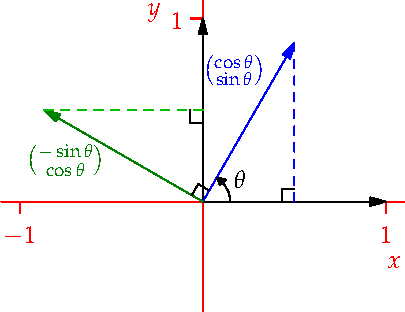
\includegraphics{moving-rot}
	  	&
	  	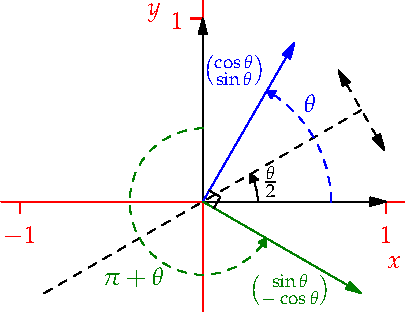
\includegraphics{moving-refl}
		\end{tabular}
	\end{enumerate}
\end{examples*}


\footnotetext{Recall that the matrix of a linear map is found by evaluating the map on the standard basis: the 1\st{} column of $A_\theta$ is the column vector $A_\theta\vi=\stwovec{\cos\theta}{\sin\theta}$. The pictures should verify the remaining columns; for $B_\theta$ you might find it helpful to consider how the required reflections of the standard basis vectors $\vi,\vj$ may be computed using \emph{rotations.}}

Motivated by the $2\times 2$ case, it is common to refer to every orthogonal matrix in $\rO_3(\R)$ as a \emph{rotation} ($\det=1$) or a \emph{reflection} ($\det=-1$).\footnote{A full analysis is more complicated. For instance, the map $\vx\mapsto E\vx$ in the first example is the composition of a reflection across a plane in $\E^3$ followed by a rotation in that plane.}\smallbreak

Part \ref*{lemm:orth3} of Lemma \ref{lemm:orth} says that multiplication by an orthogonal matrix preserves the dot product and thus (Definition \ref{defn:dotprod}) the \emph{lengths} of vectors and the \emph{angles} between them. We use this to define a useful family of transformations of $\E^3$.

\begin{defn}{}{rigid}
	An \emph{isometry} is a function $S:\E^3\to\E^3$ acting on points/position vectors by
	\[
		S(\vx)=A\vx+\vb
	\]
	where $\vb$ is a constant vector and $A\in\rO_3(\R)$. We call $S$ a \emph{direct isometry} or \emph{rigid motion} if $\det A=1$ ($A\in\rSO_3(\R)$), and an \emph{indirect isometry} otherwise.
\end{defn}

Isometry literally means \emph{equal length}; it can be seen that every function $S:\E^3\to\E^3$ which preserves distances between all pairs of points is an isometry. \emph{Congruent} geometric objects (in standard Euclidean geometry) are precisely those which are related by an isometry. 


\boldsubsubsection{Moving Frames}

Thus far we have analyzed curves with reference to the standard orthonormal basis $\epsilon=\{\vi,\vj,\vk\}$. We now replace this \emph{static} frame of reference with one that \emph{moves.} The goal is eventually to describe a special moving frame with respect to which the fundamental properties of the curve are clear.


\begin{defn}{}{moving}
	Let $\vx:I\to\E^3$ be a smooth curve. Suppose that $\ve_1,\ve_2,\ve_3$ are smooth functions on $I$ such that, for each $t\in I$,
	\begin{quote}
		$\{\ve_1(t),\ve_2(t),\ve_3(t)\}$ is a positively oriented orthonormal basis of the tangent space $T_{\vx(t)}\E^3$
	\end{quote}
	We call this family of functions a \emph{moving frame} along $\vx$.\smallbreak
	Equivalently, $E(t)=\bigl(\ve_1(t)\ \ve_2(t)\ \ve_3(t)\bigr)$ is a smooth function $E:I\to\rSO_3(\R)$. We will often refer to this matrix-valued function as a moving frame.
\end{defn}

\begin{center}
	\begin{tabular}{c@{\hspace{20pt}}c}
		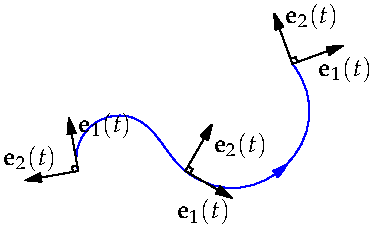
\includegraphics[scale=1]{vector-frame-e2}
		&
		\href{http://math.uci.edu/~ndonalds/math162a/vector-frame-e3.html}{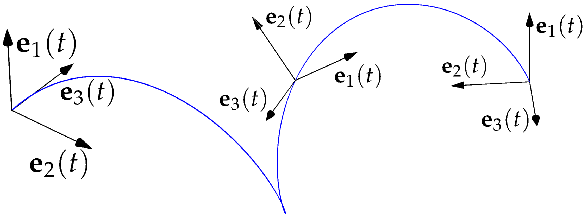
\includegraphics[scale=0.9]{vector-frame-e3}}
		\\
		A moving frame in $\E^2$&A moving frame in $\E^3$
	\end{tabular}
\end{center}

The smoothness criterion needs a little unpacking. At each point on the curve, the tangent space $T_{\vx(t)}\E^3$ has a standard basis of tangent vectors $\{\vi_{\vx(t)},\vj_{\vx(t)},\vk_{\vx(t)}\}$, with respect to which
\[
	\ve_j(t) =a_j(t)\vi_{\vx(t)}+b_j(t)\vj_{\vx(t)}+c_j(t)\vk_{\vx(t)} =\threevec{a_j(t)}{b_j(t)}{c_j(t)}
\]
We require that the functions $a_j,b_j,c_j:I\to \R$ be smooth. Strictly speaking, $\ve_j(t)$ is a \emph{smooth vector field} along the curve.


\begin{example}[lower separated=false, sidebyside, sidebyside align=top seam, sidebyside gap=0pt, righthand width=0.4\linewidth]{}{easymovingframe}
	We define a moving frame along the unit circle $\vx(t)=\bigl(\cos t,\sin t\bigr)$ via
	\[
		\ve_1(t) =\twovec{\cos 2t}{\sin 2t}\qquad \ve_2(t) =\twovec{-\sin 2t}{\cos 2t}
	\]
	Click on the picture to see how the frame rotates twice as one travels once round the circle!\smallbreak
	In accordance with the definition, for each $t$,
	\[
		E(t)=
		\begin{pmatrix}
			\cos 2t&-\sin 2t\\
			\sin 2t&\cos 2t
		\end{pmatrix}
		\in\rSO_3(\R)
	\]
	\tcblower
	\flushright\href{http://math.uci.edu/~ndonalds/math162a/vector-anim.html}{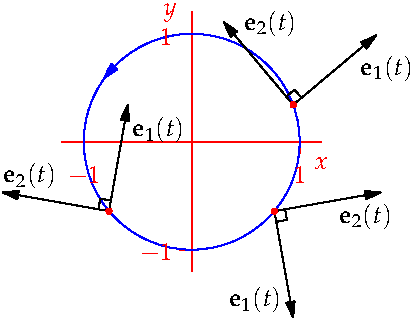
\includegraphics[scale=0.9]{vector-anim2}}
\end{example}

\goodbreak


The obvious disadvantage of a moving frame is that we have to understand how such a frame moves!

\begin{thm}{Structure equations}{moving}
	Suppose $\{\ve_1(t),\ve_2(t),\ve_3(t)\}$ is a moving frame (orthonormal positive orientation). For each $j$, express the derivative as a linear combination
	\[
		\ve_j'=\ve_1w_{1j}+\ve_2w_{2j}+\ve_3w_{3j}
	\]
	where each $w_{ij}(t) =\ve_i\cdot\ve_j'$ is a scalar function. Then the matrix $W=(w_{ij})$ is skew-symmetric:\footnotemark
	\[
		\bigl(\ve_1'\ \ \ve_2'\ \ \ve_3'\bigr)=
		\bigl(\ve_1\ \ \ve_2\ \ \ve_3\bigr)
		\begin{pmatrix}
			0&w_{12}&w_{13}\\
			-w_{12}&0&w_{23}\\
			-w_{13}&-w_{23}&0
		\end{pmatrix}
		\tag{matrix form $E'=EW$}
	\]
\end{thm}

\footnotetext{The set of skew-symmetric matrices is sometimes denoted $\fso_3(\R)$. The structure equations are an example of the relationship between a \emph{Lie group} and its \emph{Lie algebra,} a foundation on which much advanced differential geometry rests.}

In $\E^2$, there is only a single function $w_{12}=\ve_1\cdot \ve_2'$. As we've done already, we often drop the $(t)$ to make things more readable; just remember that everything is still a \emph{function}!


\begin{proof}
	Since $\ve_i\cdot\ve_j$ is constant (equals 0 or 1), the product rule says that
  \[
  	0=\diff t\bigl(\ve_i\cdot\ve_j\bigr) =\ve_i'\cdot\ve_j+\ve_i\cdot\ve_j'  \implies w_{ji}+w_{ij}=0\tag*{\qedhere}
  \]
\end{proof}

\begin{examples}{}{}
	\exstart Example \ref{ex:easymovingframe} described a moving frame in $\E^2$:
	\[
		w_{12}(t)=\ve_1(t)\cdot \ve_2'(t)=\twovec{\cos 2t}{\sin 2t}\cdot\twovec{-2\cos 2t}{-2\sin 2t}=-2
	\]
	The structure equations are therefore
	\[
		(\ve_1'\ \ve_2')=(\ve_1\ \ve_2)
		\begin{pmatrix}
			0&-2\\
			2&0
		\end{pmatrix}
	\]
	\begin{enumerate}\setcounter{enumi}{1}
		\item A moving frame can be described without mentioning a specific curve $\vx(t)$:
		\[
			\ve_1(t) =\threevec{\cos^2\!t}{\cos t\sin t}{\sin t}\qquad \ve_2(t) =\threevec{\sin t}{-\cos t}{0}\qquad \ve_3(t) =\threevec{\sin t\cos t}{\sin^2\!t}{-\cos t}
		\]
		The structure equations are easily computed
		\begin{gather*}
			w_{12}(t) =\ve_1\cdot\ve_2' =\cos^3\!t+\cos t\sin^2\!t =\cos t,\\
			w_{13}(t) =\ve_1\cdot\ve_3' =\cos^2\!t(\cos^2\!t-\sin^2\!t)+2(\cos t\sin t)^2+\sin^2\!t =1\\
			w_{23}(t) =\ve_2\cdot\ve_3' =\sin t(\cos^2\!t-\sin^2\!t)-\cos t(2\cos t\sin t) =-\sin t\\
			\begin{pmatrix}
	  		\ve_1'&\ve_2'&\ve_3'
	  	\end{pmatrix}
	  	=
			\begin{pmatrix}
				\ve_1&\ve_2&\ve_3
			\end{pmatrix}
			\begin{pmatrix}
				0&\cos t&1\\
				-\cos t&0&-\sin t\\
				-1&\sin t&0
			\end{pmatrix}
		\end{gather*}
	\end{enumerate}
\end{examples}


\begin{exercises}
	\exstart Express $\vv=\stwovec 51=a_1\ve_1+a_2\ve_2$ as a linear combination with respect to the orthonormal basis $\beta =\{\ve_1,\ve_2\} =\left\{\frac 1{13}\stwovec 5{12},\frac 1{13}\stwovec{12}{-5}\right\}$ of $\E^2$.

	\begin{enumerate}\setcounter{enumi}{1}
	  \item\begin{enumerate}
	    \item Show that $\beta=\smash[b]{\scalebox{0.8}{$\left\{\dfrac 13\threevec 221,\dfrac 1{\sqrt 2}\threevec 1{-1}0,\dfrac 1{3\sqrt 2}\threevec{-1}{-1}4\right\}$}}$ is an orthonormal basis of $\E^3$. Is it positively oriented?
	    \item Find the co-ordinates of $\smash[t]{\sthreevec 100}$ with respect to $\beta$.
	  \end{enumerate}
	  
	  
	  \item\begin{enumerate}
			\item Explain why the product rule $\diff t(\vx\cdot\vy)=\vx'\cdot\vy+\vx\cdot\vy'$ holds for differentiable curves $\vx,\vy$.    
			\item Let $\vx,\vy$ be differentiable on an interval and use the product rule to answer the following:
			\begin{enumerate}
			  \item Suppose $\vx(t_0)$ and $\vx'(t)$ are orthogonal to a fixed vector $\vv$ (the latter for all $t$). Show that $\vx(t)$ is always orthogonal to $\vv$.
				\item If $\vy(t_0)$ is a point on $\vy$ which is closest to the origin, show that $\vy(t_0)\perp\vy'(t_0)$.
			\end{enumerate}
		\end{enumerate}
	  
	  
	  \item Find the function $w_{12}$ for the moving frame $\{\ve_1,\ve_2\}=\scalebox{0.8}{$\left\{\dfrac 1{1+t^2}\twovec{2t}{1-t^2},\dfrac 1{1+t^2}\twovec{t^2-1}{2t}\right\}$}$
	  
	  
	 	\item Find the structure equations for the moving frame $\{\ve_1,\ve_2,\ve_3\} =\left\{\sthreevec{\cos t}0{\sin t}, \sthreevec 010, \sthreevec{-\sin t}{0}{\cos t}\right\}$
	  
	  
	  \item\begin{enumerate}
	    \item Explain why every moving frame in $\E^2$ has the form $\{\ve_1,\ve_2\} =\left\{\stwovec{\cos \theta(t)}{\sin \theta(t)},\stwovec{-\sin\theta(t)}{\cos \theta(t)}\right\}$ for some function $\theta$.
	    \item Find the structure equations for this frame: how does $w_{12}$ relate to $\theta$?
	    \item\label{exs:frenet2deasy} If $\vx(t)$ is parametrized at unit speed such that $\ve_1(t)=\vx'(t)$, what is $w_{12}(t)$?
	  \end{enumerate}
	  
	  
	  \item\begin{enumerate}
	    \item Let $E(t)$ be a square matrix-valued function. Show that $\diff t(E(t))^{-1}=-E^{-1}E'E^{-1}$.
			\item Suppose $E:I\to \rO_3(\R)$ is differentiable and define $W(t):=E^{-1}(t)E'(t)$. Use part (a) to prove that $W(t)$ is skew-symmetric ($W^T=-W$).
	  \end{enumerate}
	  
	  
	  \item\begin{enumerate}
	    \item Verify parts 2 and 3 of Lemma \ref{lemm:orth}.
	    \item Suppose $f,g$ are rigid motions. Show that $f\circ g$ and $f^{-1}$ are also rigid motions.
	  \end{enumerate}
	  
	  
	  \item\label{exs:tanvecrigid} Let $\vi=\stwovec 10$. Suppose $\vp\in\E^2$ and a unit vector $\vv$ are given. Prove that there is a unique rigid motion $S:\vx\mapsto A\vx+\vb$ such that
	  \[
	  	S(\V0)=\vp\quad \text{and}\quad S(\vi)=\vp+\vv
	  \]
	  Write $\vi_{\V0}=\bigl(\V0,\vi\bigr)\in T_{\V0}\E^2$ and $\vv_{\vp}=\bigl(\vp,\vv\bigr)\in T_{\vp}\E^2$ as \emph{tangent vectors,} explain why it is reasonable to write $\vv_{\vp}=S(\vi_{\V0})=(A\vi)_{\vp}$: i.e., only $A$ affects the \emph{directional part} of a tangent vector.
	  
	
		\item (Hard)\quad Suppose that a moving frame has structure equations 
		\[
			\ve'_1=-\tfrac 1{\sqrt 2}(\ve_2+\ve_3),\qquad\ve'_2=\tfrac 1{\sqrt 2}\ve_1,\qquad\ve'_3=\tfrac 1{\sqrt 2}\ve_1
		\]
		\begin{enumerate}
		  \item By considering $\ve_1''$, show that the vector $\ve_1\times\ve_1'$ is constant.
		  \item Show that $\Nm{\ve_1'}$ is constant.
		  \item Prove that there exists a constant positively oriented orthonormal basis $\{\va,\vb,\vc\}$ such that $\ve_1(t)=\cos t\va+\sin t\vb$ and compute $\ve_2,\ve_3$ in terms of this basis.
		\end{enumerate}
	% 	
	% 	\item Suppose that $\vx(t),\vy(t)$ are curves such that $\vx(t)$ is orthogonal to both $\vy(t)$ and $\vy'(t)$ for every $t$. Then,
	% 	\[\vx'(t)\cdot\vy(t)=\diff{t}(\vx(t)\cdot\vy(t))-\vx(t)\cdot\vy'(t)=0\]
	% 	so that $\vx'$ is orthogonal to $\vy$ also.
	% 
	% 	\item Suppose that $\vx(t)\times\vx'(t)=\vk$ is a constant vector. Then
	% 	\[\V0=\diff{t}(\vx\times\vx')=\vx'\times\vx'+\vx\times\vx''=\vx\times\vx''\]
	% and so $\vx''$ is parallel to $\vx$.
	
	\end{enumerate}
\end{exercises}

\clearpage



\subsection{The Frenet Frame for a Spacecurve}\label{sec:frenet}

In this section we analyze spacecurves with respect to a moving frame \emph{adapted} to the curve. To do this, we need to restrict our class of curves slightly. For this section, we work exclusively in $\E^3$.


\begin{defn}{}{}
	A regular \emph{spacecurve} $\vx:I\to\E^3$ is \emph{biregular} if it has \emph{non-zero curvature} $\kappa$.
\end{defn}

Every biregular curve is necessarily regular, but the converse is false. For instance, a straight line is regular but \emph{not biregular.} Indeed for a biregular curve, the vectors $\vx'(t)$ and $\vx''(t)$ must be linearly independent.

\begin{defn}{}{}
	Let $\vx:I\to\E^3$ be a biregular unit-speed curve. The \emph{Frenet frame} $E(t)=(\vT\ \vN\ \vB)$ is the moving frame defined as follows:
	\begin{quote}
		$\vT:=\vx'$ is the \emph{unit tangent} vector field\par
		$\vN:=\frac 1{\kappa}\vT'$ is the \emph{principal normal} vector field\par
		$\vB:=\vT\times\vN$ is the \emph{binormal} vector field
	\end{quote}
\end{defn}

We verify that the Frenet frame is indeed a moving frame:
\begin{enumerate}
  \item Since $\vx$ is unit-speed, $\vT$ has unit length.
  \item By the product rule, $\vT\cdot\vT=1\implies 2\vT'\cdot\vT=0\implies \vN\cdot\vT=0$. Moreover, the definition of curvature tells us tht
  \[\Nm{\vN}=\frac 1\kappa\Nm{\vT'}=\frac 1\kappa\Nm{\vx''}=\frac\kappa\kappa=1\]
  so that $\vN$ is a unit vector perpendicular to $\vT$.
  \item Standard properties of the cross product finish things off:
  \begin{itemize}
    \item $\vB$ has unit length since $\Nm{\vB}=\Nm{\vT}\Nm{\vN}\sin\theta =1$ ($\theta=\ang{90}$ is the angle between $\vT,\vN$).
    \item $\bigl(\vT\times\vN)\cdot\vz=\det\bigl(\vT\ \vN\ \vz\bigr)$ with $\vz=\vT$ or $\vN$ says that $\vB$ is perpendicular to $\vT,\vN$. Finally, let $\vz=\vB$ to see that the Frenet frame is positively oriented.
  \end{itemize}
\end{enumerate}


\begin{thm}{}{frenet}
	The Frenet frame is a moving frame. Its structure equations are
	\[
		\bigl(\vT'\ \ \vN'\ \ \vB'\bigr)
  	=
  	\bigl(\vT\ \ \vN\ \ \vB\bigr)
  	\begin{pmatrix}
			0&-\kappa&0\\
			\kappa&0&-\tau\\
			0&\tau&0
		\end{pmatrix}
		\qquad\qquad 
		\begin{cases}
			\vT'=\kappa\vN\\
			\vN'=-\kappa\vT+\tau\vB\\
			\vB'=-\tau\vN
		\end{cases}
  \]
	where $\kappa>0$ is the curvature and $\tau=\vN'\cdot\vB=-\vN\cdot\vB'$ is called the \emph{torsion.}
\end{thm}


The structure equations for the Frenet frame are also known as the \emph{Frenet--Serret equations.} The moving planes spanned by pairs of these vectors have special names:
\begin{quote}
	$\Span\{\vT,\vN\},\Span\{\vT,\vB\}$ and $\Span\{\vN,\vB\}$ are the \emph{osculating, rectifying} and \emph{normal} planes.
\end{quote}
At any point, the tangent line lies in the osculating plane. %The torsion describes how the osculating plane changes as we move along the curve. 


\goodbreak
	
\begin{examples}{}{frenetexs}
	\exstart We compute the Frenet frame and its structure equations for the standard helix $\vx(s)=\bigl(\cos\frac s{\sqrt 2},\sin\frac s{\sqrt 2},\frac s{\sqrt 2}\bigr)$ parametrized by arc-length (\href{http://www.math.uci.edu/~ndonalds/math162a/frenet-helixstill.html}{3D pic})(\href{http://www.math.uci.edu/~ndonalds/math162a/frenet-helixanim.html}{animation})\par
		\begin{enumerate}\setcounter{enumi}{1}
			\begin{minipage}[t]{0.71\linewidth}\vspace{-8pt}
				\item[]\begin{gather*}
				\begin{aligned}
					\vT(s)&=\vx'(s) =\frac 1{\sqrt 2}\threevec{-\sin\frac s{\sqrt 2}}{\cos\frac s{\sqrt 2}}1\implies \vT'(s)=-\frac 12\threevec{\cos\frac t{\sqrt 2}}{\sin\frac t{\sqrt 2}}0\\
					&\implies \vN(s) =-\threevec{\cos\frac t{\sqrt 2}}{\sin\frac t{\sqrt 2}}0,\quad\kappa(s) =\frac 12\\
					&\implies \vB(s) =\vT(s)\times\vN(s) =\frac 1{\sqrt 2}\threevec{\sin\frac s{\sqrt 2}}{-\cos\frac s{\sqrt 2}}1
				\end{aligned}\\
				\tau(s) =\vN'(s)\cdot\vB(s) =\frac 1{2}\threevec{\sin\frac s{\sqrt 2}}{-\cos\frac s{\sqrt 2}}0\cdot\threevec{\sin\frac s{\sqrt 2}}{-\cos\frac s{\sqrt 2}}1=\frac 12
			\end{gather*}
			The Frenet--Serret equations for the helix are therefore
			\[
				\bigl(\vT'\ \ \vN'\ \ \vB'\bigr)
				=
				\bigl(\vT\ \ \vN\ \ \vB\bigr)
				\begin{pmatrix}
		    	0&-\frac 12&0\\
					\frac 12&0&-\frac 12\\
					0&\frac 12&0
				\end{pmatrix}
			\]
		\end{minipage}
		\hfill
		\begin{minipage}[t]{0.28\linewidth}\vspace{-15pt}
			\flushright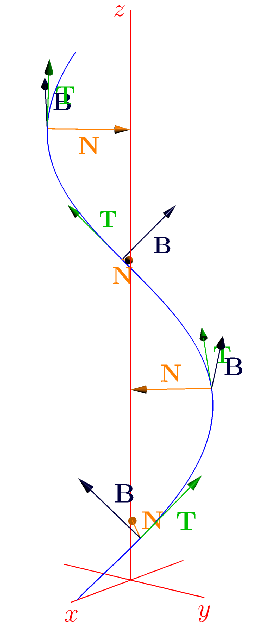
\includegraphics{frenet-helixstill}
		\end{minipage}
		\par
	
	  \item Let $\vx(s) =\bigl(\frac 13(1+s)^{3/2},\frac 1{\sqrt 2}s,\frac 13(1-s)^{3/2}\bigr)$ for $s\in(-1,1)$. First we verify this is unit-speed
		\[
			\vx'(s) =\frac 12\threevec{\sqrt{1+s}}{\sqrt 2}{-\sqrt{1-s}} \implies v(s)=\Nm{\vx'(s)} =\frac 12\sqrt{1+s+2+1-s}=1
		\]
		It follows that $\vT=\vx'$. Now compute the rest of the Frenet apparatus:
		\begin{gather*}
			\vT' =\frac 14\threevec{(1+s)^{-1/2}}0{(1-s)^{-1/2}} \implies \kappa =\Nm{\vT'} =\frac 14\sqrt{\frac 1{1+s}+\frac 1{1-s}} =\frac 1{2\sqrt 2\sqrt{1-s^2}}\\
			\vN =\frac 1{\kappa}\vT' =\frac{2\sqrt 2\sqrt{1-s^2}}4\threevec{(1+s)^{-1/2}}0{(1-s)^{-1/2}} =\frac 1{\sqrt 2}\threevec{\sqrt{1-s}}0{\sqrt{1+s}}\\
			\vB =\vT\times\vN =\frac 12\threevec{\sqrt{1+s}}{-\sqrt 2}{-\sqrt{1-s}} \implies \tau =\vN'\cdot\vB =\frac{-1}{2\sqrt 2\sqrt{1-s^2}}\\
			\bigl(\vT'\ \ \vN'\ \ \vB'\bigr)
			=\frac{\bigl(\vT\ \ \vN\ \ \vB\bigr)}{2\sqrt 2\sqrt{1-s^2}}
		  \begin{pmatrix}
				0&-1&0\\
				1&0&1\\
				0&-1&0
			\end{pmatrix}
		\end{gather*}
	\end{enumerate}

\end{examples}

         
\boldsubsubsection{The Frenet Frame in arbitrary parametrization}

Since there are relatively few curves for which an \emph{explicit} unit-speed parametrization can be found, we want to be able to compute the Frenet frame for any biregular curve, regardless of parametrization. This requires nothing more than the careful application of the chain rule\ldots

\begin{example}{}{}
	We compute for the exponential spiral $\vx(t)=\bigl(e^t\cos t,e^t\sin t,e^t\bigr)$.
	\[
		\vx'(t) =e^t\threevec{\cos t-\sin t}{\sin t+\cos t}1 \implies v(t) =\sqrt 3e^t \implies \vT(t) =\frac{1}{\sqrt 3}\threevec{\cos t-\sin t}{\sin t+\cos t}1
	\]
	Since $\vT(t)$ has unit length, $\vT'\perp\vT$. But then
	\begin{align*}
		\vT'(t) =\frac 1{\sqrt 3}\threevec{-\sin t-\cos t}{\cos t-\sin t}0 
		&\implies \vN(t) =\frac 1{\sqrt 2}\threevec{-\sin t-\cos t}{\cos t-\sin t}0 \tag{unit length $\parallel\vT'$}\\
		&\implies\vB(t) =\vT\times\vN =\frac{1}{\sqrt 6}\threevec{-\cos t+\sin t}{-\sin t-\cos t}{2}
	\end{align*}
	It is tempting to think that the curvature should be $\Nm{\vT'(t)}=\sqrt{\frac 23}$, but this is not so. Since $\vx$ is not unit-speed, we need to use the chain rule:
	\[
		\kappa =\Nm{\diff s\vT(t)} =\Nm{\diff[t]{s}\diff t\vT(t)} =\frac 1{v(t)}\Nm{\vT'(t)} =\frac{\sqrt 2}3e^{-t}
	\]
	The torsion may be computed similarly
	\[
		\tau =\diff[\vN]{s}\cdot\vB =\frac 1{v(t)}\vN'(t)\cdot\vB(t) =\frac 13e^{-t}
	\]
\end{example}

For the general result, simply(!) repeat the example in the abstract.

\begin{cor}{}{genfrenet}
	Let $\vx(t)$ be a biregular spacecurve with arbitrary parametrization. The speed, curvature, torsion, Frenet frame, and structure equations are as follows.
	\begin{gather*}
		\begin{aligned}
			&v(t)=\Nm{\vx'(t)}\qquad
			&&\kappa(t)=\frac{\Nm{\vx'\times\vx''}}{v^3}\qquad
			&&\tau(t)=\frac{(\vx'\times\vx'')\cdot\vx'''}{v^6\kappa^2}\\[8pt]
			&\vT(t)=\frac 1v\vx'\qquad
			&&\vN(t)=\frac{v\vx''-v'\vx'}{v^3\kappa}\qquad
			&&\vB(t)=\frac{\vx'\times\vx''}{v^3\kappa}
		\end{aligned}\\[8pt]
		\bigl(\vT'\ \ \vN'\ \ \vB'\bigr)
		=
		\bigl(\vT\ \ \vN\ \ \vB\bigr)
		\begin{pmatrix}
			0&-v\kappa &0\\v\kappa&0&-v\tau\\0&v\tau&0
		\end{pmatrix}
	\end{gather*}
	The curvature formula also holds if $\vx(t)$ is merely regular.
\end{cor}




\begin{exercises}
	\exstart Compute the curvature and torsion of the spiral $\vx(t)=\bigl(e^t\cos t,e^t\sin t,e^t\bigr)$ directly using the expressions in Corollary \ref{cor:genfrenet}.


	\begin{enumerate}\setcounter{enumi}{1}
		\item\label{exs:genhelixcurv} A circular helix has the form $\vx(t)=\bigl(r\cos t,r\sin t,ht\bigr)$, where $r>0$ and $h$ are constants. Find its Frenet frame and show that its curvature and torsion are given by
	  \[
	  	\kappa=\frac{r}{r^2+h^2},\qquad\tau=\frac{h}{r^2+h^2}
	  \]
	
	
		\item Find the curvature and torsion of the curve $\vx(t)=\bigl(t,t^2,t^3\bigr)$. 
	
	  
	  \item Given $\vx(t)=\frac 1{\sqrt 5}\Bigl(\sqrt{1+t^2}, 2t ,\ln\bigl(t+\sqrt{1+t^2}\bigr)\Bigr)$, find the Frenet frame, curvature and torsion.
	  
	  
	  \item Let $f(t)=\sqrt 2\int_0^t\sqrt{1-e^{-2u}}\,\du$, and define the curve $\vx(t)=\frac 1{\sqrt 2}\bigl(e^{-t}\cos t, e^{-t}\sin t, f(t)\bigr)$, $t>0$.
	  %(this is a spiral that moves upwards as it spirals towards the center of the $x,y$-plane)
	  \begin{enumerate}
	    \item Verify that $\vx(t)$ has unit speed.
	    \item Calculate the curvature of $\vx$ and show that $\lim\limits_{t\to\infty}\kappa(t)=0$.
	  \end{enumerate}
	  
	  
	  \item Let $a,b$ be positive constants and $\vx(t)=\bigl(4a\cos^3\!t, 4a\sin^3\!t, 3b\cos 2t\bigr)$ where $0<t<\frac\pi 2$. Find the Frenet frame, curvature and torsion of $\vx$.
	  
	  
	  \item Let $\vx:I\to\E^3$ be a twice-differentiable regular curve.
	  \begin{enumerate}
	    \item Prove the formula for $\kappa$ in Corollary \ref{cor:genfrenet}:
	  	\[
	  		\kappa(t)=\frac{\Nm{\vx'\times\vx''}}{v^3}
	  	\]
	  	Hence conclude that $\kappa(t_0)=0\iff\vx'(t_0)$ and $\vx''(t_0)$ are parallel.\par
			(\emph{Hint: let $\vx(t)=\vy\bigl(s(t)\bigr)$ where $\vy(s)$ has unit speed})
	  
	  	\item Prove as much else as you can tolerate of Corollary \ref{cor:genfrenet}.
	  \end{enumerate}
	
	  \item Suppose $\vx:I\to\E^3$ is a curve lying on the surface of the unit sphere ($\Nm{\vx}=1$).
	  \begin{enumerate}
	    \item If $\vx$ has unit speed, show that $\vx''\cdot\vx=-1$.
	    
	    \item Hence or otherwise, prove that the curvature of $\vx$ is at least 1 everywhere.\par
	    (\emph{Hint: $\vx$ and $\vx'$ are orthonormal\ldots})
	    
	    \item What happens if $\vx$ lies on the surface of the sphere $\Nm\vx=r$ of radius $r>0$?
	    
	    \item (Hard) If a \emph{unit-speed} curve lies on a sphere of radius $r$, show that
	    \[
	    	\tau^2(r^2\kappa^2-1)=(\kappa')^2
	    \]
	    (\emph{Hint: compute the coefficients of $\vx$ with respect to the Frenet frame})
	  \end{enumerate}
	 
	
		\item (Hard)\quad Let $d(t)>0$. Suppose $\vx(t)$ and $\vy(t)=\vx(t)+d\vN(t)$ are unit-speed curves such that the principal normal vector field $\vN$ of $\vx$ is the translate\footnote{That is, the directional parts of $\vN,\hat\vB$ are identical: of course these are members of different tangent spaces.} of the binormal vector field $\hat\vB$ of $\vy$.\par
		Prove that the distance $d$ between corresponding points of the curves is \emph{constant.} Prove also that the curvature and torsion of $\vx$ satisfy $2\kappa=d(\kappa^2+\tau^2)$.\par
		(\emph{Hint: Compute $\hat\vT$ and take dot products with something useful\ldots})
	  
	\end{enumerate}
\end{exercises}

\clearpage



\subsection{The Fundamental Theorem of Biregular Spacecurves}


Our goal for this section is to see that curvature and torsion determine a spacecurve uniquely up to rigid motions. We do this by recognizing the Frenet--Serret equations satisfied by the Frenet frame as a system of ordinary differential equations; provided sufficient initial conditions (starting point and orientation), the usual existence and uniqueness theorem for initial value problems shows that there is a unique curve with this data.\medbreak

As a precursor, we consider how to interpret curvature and torsion, and how they change (or don't!) under rigid motions of a curve.

\begin{thm}{}{curvtormeaning}
	\exstart A regular spacecurve has $\kappa\equiv 0$ if and only if it is a straight line.
	\begin{enumerate}\setcounter{enumi}{1}
	  \item A biregular spacecurve has $\tau\equiv 0$ if and only if it is contained in a fixed plane (the unmoving osculating plane of the curve).
	\end{enumerate}
\end{thm}

\begin{proof}
	In both cases, we assume, without loss of generality, that $\vx(s)$ is a unit-speed parametrization of our spacecurve.
	\begin{enumerate}
	  \item $\kappa(s)=\Nm{\vx''(s)}=0\iff\vx''(s)=\V0$. Thus $\vx$ is a straight line.
	  \item ($\Leftarrow$)\quad Suppose the curve lies in a fixed plane. Then $\vx'$ and $\vx''$ are parallel to this plane, whence $\vT$ and $\vN$ are also. But then $\vB$ is a continuous unit vector orthogonal to the plane and is therefore \emph{constant.} From the Frenet equations, $-\tau\vN=\vB'=\V0\implies \tau\equiv 0$.\par
	  ($\Rightarrow$)\quad As above, if $\tau\equiv 0$, then $\vB$ is constant. But then
	  \[
	  	(\vx\cdot\vB)'=\vx'\cdot\vB+\vx\cdot\vB'=\vT\cdot\vB=0
	  \]
	  from which $\vx\cdot\vB$ is constant. The curve therefore lies in a fixed plane perpendicular to $\vB$.\qedhere
	\end{enumerate}
\end{proof}


Curvature measures the deviation of a curve from a straight line; its \emph{bending.} Torsion measures how badly a curve fails to be planar; its \emph{twisting.}\smallbreak

To visualize the difference, the pictures below show a segment of a standard helix. In the first we look down the binormal onto the \textcolor{blue}{osculating plane}; the non-zero curvature is clearly visible. In the second we look along the principal normal vector $\vN$ and across the osculating plane; the positive torsion ($\tau=\frac 12$) indicates that the curve crosses the plane similarly to how the cubic function $y=x^3$ crosses the $x$-axis. The full 3D curve is linked via either picture.


\begin{center}
\href{http://www.math.uci.edu/~ndonalds/math162a/frenet-helixstill3.html}{
	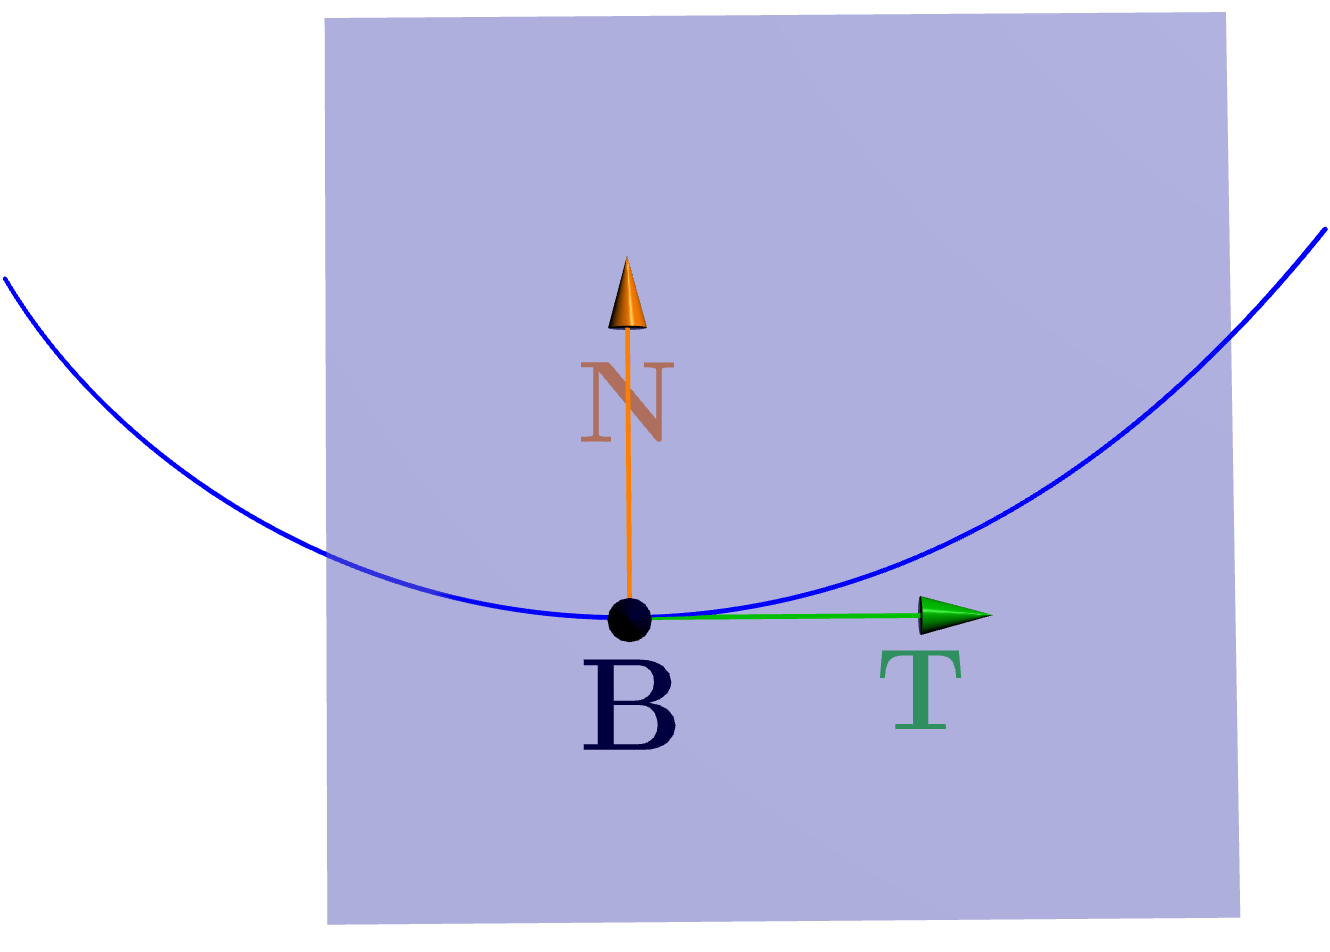
\includegraphics[scale=0.12]{frenet-helixstill3.png}
	\qquad
	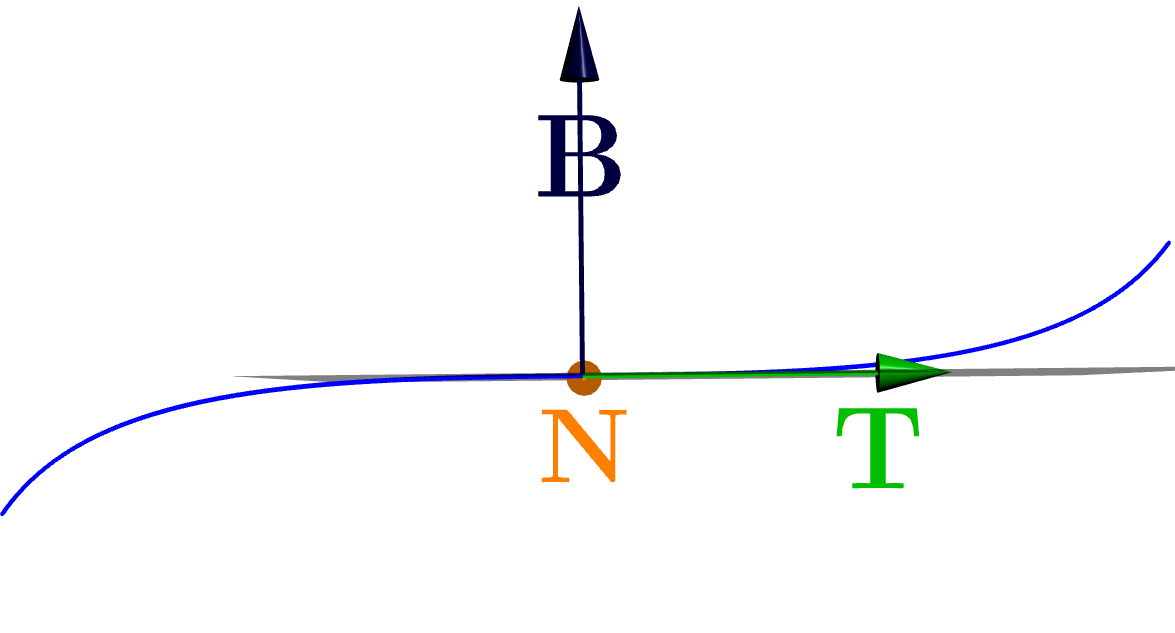
\includegraphics[scale=0.18]{frenet-helixstill3a.png}
	}
\end{center}

\clearpage


\begin{thm}{}{isometrytrans}
	Under an isometry $\hat{\vx}:=A\vx+\vb$ (recall Definition \ref{defn:rigid}), the curvature and torsion of a biregular spacecurve transform as follows:
	\begin{enumerate}
		\item[]Direct isometry/rigid motion:\quad $\hat{\kappa}=\kappa,\quad\hat{\tau}=\tau$.
		\item[]Indirect isometry:\quad $\hat{\kappa}=\kappa,\quad\hat{\tau}=-\tau$.
	\end{enumerate}
\end{thm}

\begin{proof}
	Suppose $\vx(s)$ has unit-speed. We relate the Frenet frame $(\hat\vT\ \hat\vN\ \hat\vB)$ of $\hat\vx$ to the original.\footnotemark\smallbreak
	Since orthogonal matrices preserve the dot  product (Lemma \ref{lemm:orth}), $\hat\vx$ has unit-speed also:
	\[
		\hat\vx'(s) =A\vx'(s)\implies \hat v(s) =\Nm{\hat\vx'(s)} =\Nm{\vx'(s)} =1 \implies \hat\vT =A\vT
		\]
	Moreover, since $A$ is constant and both $\hat\vN$ and $\vN$ have unit length,
	\[
		\frac 1{\hat\kappa}\hat\vN =\hat\vT'=A\vT' =\frac 1\kappa A\vN \implies \hat\kappa=\kappa \quad\text{and}\quad \hat\vN=A\vN
	\]
	Curvature is therefore invariant under any isometry. Since $A$ preserves angles, $A\vB$ is perpendicular to both $\hat\vT$ and $\hat\vN$, and so $A\vB=\pm\hat\vB$. Since the Frenet frame $E=(\vT\ \vN\ \vB)$ is a special orthogonal matrix, $AE$ is also orthogonal, and moreover
	\[
		\det AE=\det A\det E=\det A
	\]
	We conclude that $\det A=1\iff AE=(A\vT\ A\vN\ A\vB) =(\hat\vT\ \hat\vN\ A\vB)$ is \emph{positively oriented,} whence
	\[
		\hat\vB=(\det A)A\vB=
		\begin{cases}
	  	A\vB&\text{ if the isometry is direct,}\\
			-A\vB&\text{ if the isometry is indirect.}
		\end{cases}
	\]
	Finally, we compute the torsion:
	\[
		\hat\tau=\hat\vN'\cdot\hat\vB= A\vN'\cdot\bigl((\det A)(A\vB)\bigr)= (\det A)(A\vN')\cdot(A\vB) =(\det A)\vN'\cdot\vB=(\det A)\tau \tag*{\qedhere}
	\]
\end{proof}


\footnotetext{Recall Exercise \ref*{sec:orth}.\ref{exs:tanvecrigid}: when we write $\hat\vT=A\vT$ we mean that the \emph{directional parts} of the tangent vectors are thus related.}


\boldsubsubsection{Existence and Uniqueness of Solutions to ODEs}


Our classification of spacecurves depends on the `usual' existence and uniqueness result for ODEs. Here is a version suitable for our needs.
% 
% \begin{thm}{Picard, Lindelöf, etc.}{}
% Let $a\in\R$ and $\vc\in\R^n$ be fixed. Let $\V F(\vx,t)$ be a continuous vector-valued function defined on some closed region
% \[\nm{\vx-\vc}\le K\quad\text{and}\quad \nm{t-a}\le T\]
% and suppose that the partial derivatives of $\V A$ with respect to the co-ordinates of $\vx$ are bounded.\footnote{The requirement that the partial derivatives be bounded may be relaxed. The technical term is that the function $\V F(\vx,t)$ be \emph{Lipshitz continuous} which essentially says that $\nm{\V F(\vx,t)-\V F(\vy,t)}\le B\nm{\vx-\vy}$ for some constant $B$.} Suppose also that $M=\sup\nm{\V F(\vx,t)}$ on the closed region. Then the initial value problem
% \[\begin{cases}
% \displaystyle\diff[\vE]{t}=\V F(\vE,t)\\
% \vE(a)=\vc
% \end{cases}\]
% has a unique solution $\V E:I\to \R^n$ on the interval defined by $\nm{t-a}\le\min\left(T,\frac KM\right)$.
% \end{thm}
% 
% The proof is beyond the difficulty of this course as it depends crucially on ideas from topology. The rough idea is that we produce a sequence of functions
% \[\vF_1(t)=\vc,\qquad \vF_2(t)=\vc+\int_a^t\V A(\vF_1(\tilde t),\tilde t)\D\tilde t ,\qquad \vF_3(t)=\vc+\int_a^t\V A(\vF_2(\tilde t),\tilde t)\D\tilde t,\ldots\]
% which are then shown to converge to the required solution. 
% 
% 
% \begin{cor}{}{picard}
% If the ODE in Picard's Theorem is \emph{linear} that is if $\V A(\vx,t)=A(t)\vx+\vb(t)$ for some matrix valued-function $A(t)$ and vector-valued $\vb(t)$, then the unique solution is defined on $\nm{t-a}\le T$.
% \end{cor}
% 
% \begin{proof}
% Since the only dependence of $\V A$ on $\vx$ is through multiplication, it follows that $\V A$ is continuous for all $\vx\in\R^n$. Essentially $K$ can be taken to be arbitrarily large: $K=MT$ is sufficient for the result. 
% \end{proof}

\begin{thm}{Existence/Uniqueness for Linear ODE (Picard, Lindelöf, etc.)}{}\phantom{bob}\par
	Let $t_0\in\R$ and $\vc\in\R^n$ be given, and let $M(t)\in M_n(\R)$ be a continuous matrix-valued function defined on an interval $\nm{t-t_0}\le T$. Then the initial value problem
	\[
		\diff[\vE]{t}=M(t)\vE,\qquad \vE(t_0)=\vc
	\]
	has a unique solution $\vE:[t_0-T,t_0+T]\to \R^n$.
\end{thm}

\goodbreak

The rough idea of the proof is to define a sequence of functions
\[
	\vE_0(t):=\vc,\qquad \vE_1(t):=\vc+\int_{t_0}^tM(u)\vE_0(u)\,\du,\qquad \vE_2(t):=\vc+\int_{t_0}^tM(u)\vE_1(u)\,\du,\ \ldots
\]
which are seen to converge to the required solution; this last step requires advanced ideas from topology/analysis. A simple example should convince you of the approach.

\begin{example}{}{picarditer}
	Given the initial value problem $\diff[E]{t}=2tE$, \ $E(0)=1$, we obtain
	\begin{gather*}
		E_0(t)=1,\quad E_1(t)=1+\int_0^t 2u\,\du=1+t^2,\quad
		E_2(t)=1+\int_0^t2u(1+u^2)\,\du =1+t^2+\frac 12t^4,\ldots
	\end{gather*}
	The \emph{Picard iteration} builds up the correct solution as a power series
	\[
		E(t)=e^{t^2}=\smash[t]{\sum\limits_{n=0}^\infty\frac{t^{2n}}{n!}}=1+t^2+\frac 12t^4+\frac 16t^6+\cdots
	\]
\end{example}



\begin{cor}{}{picard2}
	Let $\mathcal O$ be an orthogonal matrix, $I=[t_0-T,t_0+T]$ an interval, and $W:I\to M_3(\R)$ a matrix-valued function such that each $W(t)$ is \emph{skew-symmetric.}  Then:
	\begin{enumerate}\itemsep0pt
	  \item There exists a unique solution $E:I\to \rO_3(\R)$ to the initial value problem
	  \[
	  	\diff[E]{t}=E W,\qquad E(t_0)=\mathcal O
	  \]
	  \item If $\det\mathcal O=1$, then $E:I\to\rSO_3(\R)$.
	\end{enumerate}
\end{cor}

\begin{proof}
	\begin{enumerate}
	  \item The initial value problem is a system of nine linear first order ODEs in the entries of the $3\times 3$ matrix $E$. We are therefore in the case of Picard's theorem where $\vE:I\to\R^9$. There therefore exists a unique solution $E:I\to M_3(\R)$. Now differentiate:
	  \begin{align*}
	  	\diff t(EE^T)&=E'E^T+E(E')^T =EWE^T+E(EW)^T =EWE^T+EW^TE^T\\
	  	&=EWE^T+E(-W)E^T=0 \tag{$W^T=-W$!}
	  \end{align*}
	  Thus $EE^T$ is constant. However $E(t_0)E(t_0)^T=\mathrm I$ since $E(t_0)=\mathcal O$ is orthogonal. We conclude that $E(t)$ is always orthogonal.
	  \item Determinant is continuous (it is a polynomial!); $E$ is differentiable, and so $\det E:I\to\R$ is continuous on an interval. But $\det E=\pm 1$ since $E$ is orthogonal. It follows that $\det E$ is the constant 1.\qedhere
	\end{enumerate}
\end{proof}

For simple $W$, we might be able to state the solution using the matrix exponential; for instance
\[
	W\text{ constant }\implies E(t)=\mathcal Oe^{tW}
\] 
This is of limited utility: the matrix exponential is rarely computable except as an infinite series, and the approach fails for general $W(t)$.

%It works if $W(t)=\alpha(t)X$ is a multiple of a constant matrix $X$, then $E(t)=\mathcal O\exp\left((\int_{t_0}^t\alpha)X\right)$. 

\begin{cor}{Fundamental theorem of biregular spacecurves}{fundcurve}\phantom{bob}\par
	Suppose we are given the following data:
	\begin{itemize}
	  \item Smooth functions $\kappa>0$ and $\tau$ on an interval $I=[t_0-T,t_0+T]$.
	  \item A position vector $\vc\in\E^3$ and a positively oriented orthonormal basis $(\vT_0\ \vN_0\ \vB_0)$ of $T_{\vc}\E^3$.
	\end{itemize}
	Then there exists a unique unit-speed biregular spacecurve $\vx:I\to\E^3$ with curvature $\kappa$, torsion $\tau$, initial position $\vx(t_0)=\vc$ and Frenet frame $E(t_0)=(\vT_0\ \vN_0\ \vB_0)$ at $\vx(t_0)$.
\end{cor}


\begin{proof}
	The structure equations $E'=EW$ put us in the situation of Corollary \ref{cor:picard2}; there exists a unique solution $E=(\vT\ \vN\ \vB):I\to\rSO_3(\R)$. Integrate the unit tangent vector field to finish:
	\[
		\vx(t)=\vc+\int_{t_0}^t\vT(u)\,\du
	\]
	This is plainly the unique curve with the required initial conditions, curvature and torsion.
\end{proof}


Alternatively, a biregular curve is determined up to rigid motions by its curvature and torsion.

\begin{cor}{}{fund2}
	Given two biregular spacecurves with the same curvature and torsion functions, there exists a unique direct isometry transforming one to the other.
\end{cor}

\begin{proof}
	Suppose $\vx_1:I\to\E^3$ and $\vx_2:I\to\E^3$ have Frenet frames $E_1,E_2$, and the same curvature and torsion functions. Choose some (any!) $t_0\in I$. The required rigid motion $S:\vx\mapsto A\vx+\vb$ must satisfy the conditions at $t_0$, whence\footnotemark
	\[
		S\bigl(\vx_1(t_0)\bigr)=\vx_2(t_0)\quad\text{and}\quad AE_1(t_0)=E_2(t_0)
	\]
	Plainly $A=E_2(t_0)\bigl(E_1(t_0)\bigr)^{-1}$ and $\vb=\vx_2(t_0)-A\vx_1(t_0)$ provide the unique isometry $S$. Moreover $\det A=1$ since both $E_1$ and $E_2$ do so also.\smallbreak
	By Theorem \ref{thm:isometrytrans}, $\vx_3:=S(\vx_1)$ is a spacecurve with the \emph{same} initial conditions (at $t_0$), curvature and torsion as $\vx_2$. The Fundamental Theorem says that $\vx_2=\vx_3=S(\vx_1)$.
\end{proof}

\footnotetext{As in Theorem \ref{thm:isometrytrans}, $S$ acts on \emph{position vectors} but Frenet frames consist of \emph{tangent vectors} and thus only see $A$.}

Compare what we've done to the standard acceleration/position kinematics problem, where \emph{three scalar functions} $\vx''(t)=\bigl(x''(t),y''(t),z''(t)\bigr)$ and \emph{six scalar initial conditions} $\vx(t_0)$ and $\vx'(t_0)$ recover the motion by twice integrating.\smallbreak
The Fundamental Theorem says that a spacecurve is determined uniquely by \emph{three scalar functions} $v(t),\kappa(t),\tau(t)$ and the \emph{initial conditions} $\vx(t_0),\vT(t_0),\vN(t_0)$, which also amount to \emph{six} scalar constants.\footnote{You don't need explicitly to specify $\vB(t_0)=\vT(t_0)\times\vN(t_0)$! The position $\vx(t_0)$ requires three constants; $\vT(t_0)$ needs two angles (spherical polar co-ordinates), and $\vN(t_0)$ a single angle in the plane $(\vT(t_0))^\perp$.}\smallbreak
One benefit of our result is that, by standardizing $v(t)\equiv 1$ and ignoring rigid motions, we see that the \emph{physical shape} of a curve depends only on \emph{two} scalar functions $\kappa(t)$ and $\tau(t)$.\bigbreak


\goodbreak

We finish this discussion with a quick application of the Fundamental Theorem.

\begin{cor}{}{}
	Every biregular curve with $\kappa$ and $\tau$ constant is a circular helix (circle if $\tau\equiv 0$).
\end{cor}

\begin{proof}
	By (Exercise \ref*{sec:frenet}.\ref{exs:genhelixcurv}), the circular helix $\vx(t)=\bigl(r\cos t,r\sin t,ht\bigr)$ has constant curvature $\kappa=\frac r{r^2+h^2}$ and torsion $\tau=\frac h{r^2+h^2}$.\smallbreak
	Given constant $\kappa,\tau$, it is a simple exercise to find suitable $r,h$. By Corollary \ref{cor:fund2}, this is the \emph{only} such curve up to direct isometry (and constant speed re-parametrization).
\end{proof}


\boldsubsubsection{What changes in other dimensions?}

For plane curves things are a little simpler. Here is a summary. 
\begin{description}
	\item[\normalfont\emph{Assumptions}] $\vx:I\to\E^2$ is regular; we don't need biregularity.
	
	\item[\normalfont\emph{Frenet frame}] $\vT:=\frac 1{v}\vx'$ and $\vN:=J\vT$ where $J=\begin{smatrix}
		0&-1\\1&0	
	\end{smatrix}$ is rotation by \ang{90} counter-clockwise; no differentiation is required to compute $\vN$!
	
	\item[\normalfont\emph{Curvature}] $\kappa=\frac 1v\vT'\cdot\vN$ is \emph{signed} as we saw in Section \ref{sec:arclength}:
	\begin{center}
		\begin{tabular}{c@{\qquad\qquad}c}
			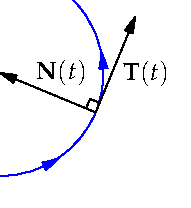
\includegraphics{fund-e2}&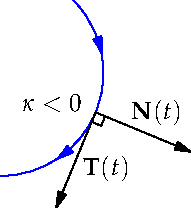
\includegraphics{fund-e2a}\\
			$\kappa>0\iff \vx$ bends towards $\vN$
			&
			$\kappa<0\iff \vx$ bends away from $\vN$
		\end{tabular}
	\end{center}
	
	\item[\normalfont\emph{Frenet--Serret equations}] In arbitrary parametrization
	$\bigl(\vT'\ \ \vN'\bigr)
  =
	\bigl(\vT\ \ \vN\bigr)
	\begin{pmatrix}
		0&-v\kappa\\
		v\kappa&0
	\end{pmatrix}
	$
	
	\item[\normalfont\emph{Isometries}] Direct isometries preserve curvature, indirect isometries change its sign.
	
	\item[\normalfont\emph{Fundamental Theorem}] Given $\kappa(s)$, $\vx(s_0)\in\E^2$ and $\vT_0\in T_{\vx(s_0)}\E^2$, there exists a unique unit-speed curve with curvature $\kappa(s)$ and these initial data. In this case we can prove the Theorem in a more elementary fashion (Exercise \ref{exs:fundthm2}).
\end{description}


\begin{minipage}[t]{0.62\linewidth}\vspace{0pt}
	We can also play this game in higher dimensions. Given a unit-speed curve $\vx:I\to\E^n$ whose first $n-1$ derivatives at each point are linearly independent, apply Gram-Schmidt orthogonalization to obtain a moving frame $E=(\ve_1\ \cdots\ \ve_n)$ and functions $\kappa_1,\ldots,\kappa_{n-1}$ (the generalized curvatures) satisfying the structure equations shown.
\end{minipage}
\hfill
\begin{minipage}[t]{0.35\linewidth}\vspace{0pt}
	\flushright$E'=E
	\begin{smatrix}
		0&-\kappa_1&0&\cdots&0&0\\
		\kappa_1&0&-\kappa_2&&0&0\\
		0&\kappa_2&0&&0&0\\
		\vdots&&&\ddots&&\vdots\\
		0&0&0&&0&-\kappa_{n-1}\\
		0&0&0&\cdots&\kappa_{n-1}&0
	\end{smatrix}$
\end{minipage}\medbreak

Conversely, the $n-1$ generalized curvatures determine the curve up to rigid motions.

\clearpage

\begin{exercises}
	\exstart Find an explicitly parametrized curve with constant curvature $\kappa$ and torsion $\tau$.
	
	\begin{enumerate}\setcounter{enumi}{1}
	  \item Reflection in the $xy$-plane $S(\vx)=\smash[t]{
		  \begin{smatrix}
				1&0&0\\
				0&1&0\\
				0&0&-1
			\end{smatrix}
		}\vx$ is an indirect isometry. Explicitly compare the curvature and torsion of the standard helix $\vx(t)=\bigl(\cos t,\sin t,t\bigr)$ with those of $S(\vx)$.
	
	
		\item In the manner of Example \ref{ex:picarditer}, compute the Picard iteration process up to $\vE_3(t)$ for the initial value problem
		\[
			\diff[\vE]{t}=
			\begin{pmatrix}
	  		0&-1\\
	  		1&0
	  	\end{pmatrix}
	  	\!\vE,\quad \vE(0)=\twovec 10
	  \]
	  Verify that this comports with the correct solution $\vE(t)=\stwovec{\cos t}{\sin t}$to this system of ODEs.
	
	  
	  \item Suppose $f$ is a function such that $\vx(t)=\bigl(\cos t,\sin t,f(t)\bigr)$ lies  in a fixed plane. Show that $f$ satisfies the 3\rd-order linear ODE $f'''(t)+f'(t)=0$ and thus find all possible functions $f$.\par
	  (\emph{Hints: What is the torsion of a plane curve?})
	  
	  
		\item Assume that all principal normals of a biregular curve in $\E^3$ pass through a fixed point: $\exists\alpha(t)$ and a constant $\vn$ such that $\vx(t)+\alpha(t)\vN(t)=\vn$. Show that the curve is (part of) a \emph{circle}.
	  
	  
	  \item Let $\vx:I\to \E^2$ be a regular curve and let $\vy=S(\vx)=A\vx+\vb$ be a new curve resulting from a rigid motion. Prove that the curvatures of $\vx$ and $\vy$ are identical.

	   
		\item\label{exs:fundthm2} For regular curves in $\E^2$, the Fundamental Theorem is relatively simple to prove.
		\begin{enumerate}
		  \item Suppose you are given a smooth function $\kappa:I\to\R$ on an interval $I$ containing $t_0$, an initial position $\vx(t_0)=(a,b)$ and an initial direction $\theta(t_0)=\theta_0$ (angle with positive $x$-axis).\par
			Use the Fundamental Theorem of Calculus to describe the unique unit-speed curve $\vx:I\to\E^2$ with curvature $\kappa$ and given initial data.\par
			(\emph{Hints: use $\theta(t):=\theta_0+\int_{t_0}^t\kappa(u)\,\du$ to define $\vT(t)$ and integrate! Your answer will contain definite integrals.})
			
			\item Suppose $\vx:\R\to\E^2$ is unit-speed with $\kappa(t)=\frac 1{1+t^2}$, $\vx(0)=(0,0)$, and $\vx'(0)=(1,0)$. Find $\vx(t)$.
		\end{enumerate}
		
	
	  \item (Hard)\quad A \emph{cylindrical helix} is a curve $\vx(t)$ whose unit tangent field $\vT(t)$ makes a constant angle $\theta\in(0,\frac\pi 2)$ with a fixed vector $\vn$.
		\begin{enumerate}
		  \item If $\vx(t)=\bigl(\cos t,\sin t,t\bigr)$ is the standard circular helix, describe a suitable vector $\vn$.
		  \item Use the Frenet--Serret formulas to prove that a (unit-speed) non-planar curve is a cylindrical helix if and only if $\kappa/\tau$ is constant.
	  \end{enumerate}
	  
	  \item (Very hard)\quad Suppose a moving frame $\ve_1,\ve_2,\ve_3$ has structure equations where all three functions $w_{12},w_{13},w_{23}$ are constant. Find the moving frame $\vf_1,\vf_2,\vf_3$ where $\vf_1=\ve_1$ such that $\vf_1,\vf_2,\vf_3$ is the Frenet frame of a unit-speed circular helix. Calculate the curvature $\kappa$ and torsion $\tau$ of this helix in terms of $w_{12},w_{13},w_{23}$. Can you find an orthogonal matrix $A$ such that
	  \[
	  	A^{-1}
	  	\begin{pmatrix}
		     0&w_{12}&w_{13}\\
		     -w_{12}&0&w_{23}\\
		     -w_{13}&-w_{23}&0
	     \end{pmatrix}
	     A=
	     \begin{pmatrix}
		     0&-\kappa&0\\
		     \kappa&0&-\tau\\
		     0&\tau&0
	     \end{pmatrix}
	     \ ?
	   \]
	\end{enumerate}
\end{exercises}


\clearpage




\subsection{Radii of curvature}\label{sec:radii}

We have seen how curvature measures the deviation of a curve from a straight line and that the only planar curves with constant curvature $\kappa$ are circles of radius $\frac 1\kappa$. We could have started with this as our definition; at a given point, a curve has curvature $\kappa$ if the circle which best approximates the curve has radius $\frac 1\kappa$. Of course, we have to define what is meant by \emph{best approximation.}

\begin{defn}{}{}
	Unit-speed curves $\vx,\vy$ have \emph{$n\th$ order contact} at an intersection point $\vx(t_0)=\vy(s_0)$, if their first $n$ derivatives agree there: $\vx^{(j)}(t_0)=\vy^{(j)}(s_0)$ for all $1\le j\le n$.
\end{defn}

\begin{minipage}[t]{0.65\linewidth}\vspace{0pt}
	Let $\vx(t)$ be a unit-speed curve in $\E^2$, fix $r\neq 0$ and consider the unit-speed circle $\vc(s)$ with (signed) radius $r$ for which
	\[
		\vc(0)=\vx(t_0) \quad\text{and}\quad \vc'(0)=\vx'(t_0)
	\]
	We take $r>0\iff$ the circle lies on the same side of the curve as the principal normal vector $\vN$.\medbreak
	The circle is straightforward to parametrize:
	\[
		\vc(s)=\underbrace{\vx(t_0)+r\vN(t_0)}_{\text{center}} +\underbrace{r\sin(s/r)\vT(t_0)-r\cos(s/r)\vN(t_0)}_{\text{rotation}}
		\]
\end{minipage}
\hfill
\begin{minipage}[t]{0.34\linewidth}\vspace{0pt}
	\flushright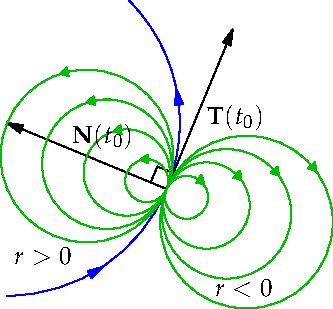
\includegraphics[scale=0.9]{radii-circles}
\end{minipage}\medbreak
Certainly this circle has 1\st-order contact with the curve: $\vc(0)=\vx(t_0)$ and 
\[
	\vc'(s)=\cos(s/r)\vT(t_0)+\sin(s/r)\vN(t_0)\implies \vc'(0)=\vT(t_0)=\vx'(t_0)
\]
Moreover,
\[
	\vc''(s)=-\frac 1r\sin(s/r)\vT(t_0)+\frac 1r\cos(s/r)\vN(t_0)\implies \vc''(0)=\frac 1r\vN(t_0)
\]
The circle has second-order contact with the curve if and only if
\[
	\vc''(0)=\vx''(t_0)\iff \frac 1r=\kappa(t_0)
\]

There is nothing stopping us from finding this circle for an arbitrary speed regular curve, since all we need is the curvature and the Frenet frame at the relevant point.

\begin{defn}{}{}
	Let $\vx(t)$ be a regular curve. At a point $\vx(t_0)$ with non-zero curvature:
	\begin{itemize}\itemsep0pt
	  \item The \emph{radius of curvature} is $r=\frac 1{\kappa(t_0)}$.
	  \item The \emph{center of curvature} is the point with position vector $\vx(t_0)+r\vN(t_0)$.
		\item The \emph{osculating circle} is the radius $r$ circle centered at the center of curvature. It has unit-speed parametrization
		\[
			\vc(s)=\vx(t_0) +\frac 1{\kappa(t_0)}\bigl(\sin(s/r)\vT(t_0) +(1-\cos(s/r))\vN(t_0)\bigr)
		\]
	\end{itemize}
\end{defn}

\emph{Osculating} means `kissing.' If $\kappa(t_0)=0$, some consider the tangent line to be an osculating circle with infinite radius!


\goodbreak

\begin{example}{}{evolparabola}
	We find the osculating circles for the parabola $y=x^2$ parametrized in the obvious manner $\vx(t)=\bigl(t,t^2\bigr)$. The relevant ingredients are
	\begin{gather*}
		\vx'(t)=\twovec{1}{2t}\implies \vT(t)=\frac 1{\sqrt{1+4t^2}}\twovec 1{2t} \qquad \vN(t)=\frac{1}{\sqrt{1+4t^2}}\twovec{-2t}{1}\\
		\vx''(t)=\twovec{0}{2},\qquad \kappa(t)=\frac 2{(1+4t^2)^{3/2}}
	\end{gather*}
	\begin{minipage}[t]{0.59\linewidth}\vspace{0pt}
		The center of curvature when $t=t_0$ has position vector
		\[
			\vx(t_0)+\frac{1}{\kappa(t_0)}\vN(t_0)=%\twovec{t_0}{t_0^2}+\frac{1+4t_0^2}{2}\twovec{-2t_0}{1}=
			\twovec{-4t_0^3}{\frac 12+3t_0^2}
		\]
		Several osculating circles are drawn and their centers of curvature indicated.
	\end{minipage}
	\hfill
	\begin{minipage}[t]{0.40\linewidth}\vspace{-35pt}
		\flushright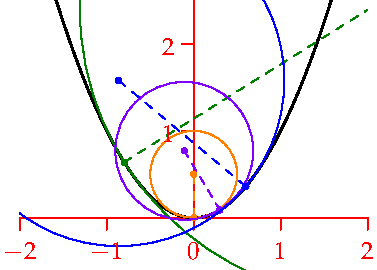
\includegraphics[scale=1]{radii-osculating3}
	\end{minipage}
\end{example}


The centers of curvature describe a curve that is interesting in its own right.

\begin{defn}{}{}
	Let $\vx(t)$ be a regular plane curve with non-zero curvature. The curve $\ve(t)$ defined by the centers of curvature is the \emph{evolute} of $\vx(t)$:
	\[
		\ve(t)=\vx(t)+\frac 1{\kappa(t)}\vN(t)
	\]
\end{defn}

\begin{example*}[lower separated=false, sidebyside, sidebyside align=top seam, sidebyside gap=0pt, righthand width=0.49\linewidth]{\ref{ex:evolparabola} cont}{}
	The evolute of the parabola $\vx(t)=(t,t^2)$ was found above:
	\[
	\textcolor{Green}{\ve(t)} =\textcolor{blue}{\vx(t)} +\frac 1{\kappa(t)}\vN(t) =\twovec{-4t^3}{\frac 12+3t^2}
	\]
	Alternatively, this is the graph $y=\frac 12+3\left(\frac x4\right)^{2/3}$: notice that this isn't regular at $x=0$.\smallbreak
	The picture now animates to show the osculating circles and the construction of the evolute.
	\tcblower
	\flushright
	\href{http://math.uci.edu/~ndonalds/math162a/radii-evolute.html}{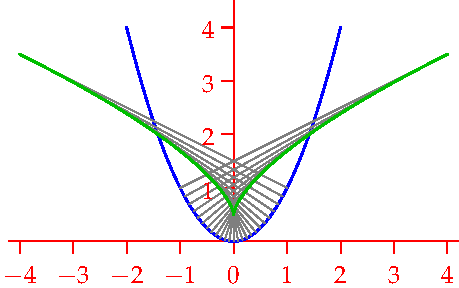
\includegraphics[scale=1]{radii-evolute2}}
\end{example*}

The gray lines are the \emph{normal lines} to the parabola, and are also \emph{tangent} to the evolute.
\[
	\ve'=\vx'-\frac{\kappa'}{\kappa^2}\vN+\frac 1\kappa(-v\kappa\vT)=-\frac{\kappa'}{\kappa^2}\vN
\]
This last means that the evolute is a \emph{focal curve} for the family of normal lines. The same equation shows that the evolute is regular precisely when $\kappa'(t)\neq 0$. 

\vfil

\goodbreak


A related notion is the \emph{involute,} which may be imagined by rolling a line along a curve and seeing what curve the end of the line traces out.

\begin{defn}{}{}
	Suppose $\vx(t)$ has unit speed. Its \emph{involute} is the curve
	\[
		\vi(t):=\vx(t)-t\vx'(t)=\vx(t)-t\vT(t)
	\]
\end{defn}

An involute depends crucially on its parametrization: it intersects its source curve when $t=0$.

\begin{examples}{}{tractrix}
	\exstart The unit speed unit circle $\vx(t)=\bigl(\cos t,\sin t\bigr)$. Its involute is therefore
	\[
		\vi(t)=\vx(t)-t\vT(t)=\twovec{\cos t+t\sin t}{\sin t-t\cos t}
	\]
	\begin{enumerate}\setcounter{enumi}{1}
  	\item\label{ex:tractrix1} The involute of the unit speed \emph{catenary} $\vx(t)=\bigl(\sinh^{-1}\!t,\sqrt{1+t^2}\bigr)$ is the \emph{tractrix}:
		\[
			\vi(t)=\twovec{\sinh^{-1}\!t-t(1+t^2)^{-1/2}}{(1+t^2)^{-1/2}}
		\]
		This is the curve obtained when an \textcolor{Green}{object} starting at the point $(0,1)$ is dragged (subjected to \emph{traction}) by attaching a \textcolor{orange}{rope} of length 1 to a vehicle moving along the $x$-axis.
		\begin{center}
			\begin{tabular}{c@{\qquad\qquad}c}
				\href{http://math.uci.edu/~ndonalds/math162a/radii-invcirc.html}{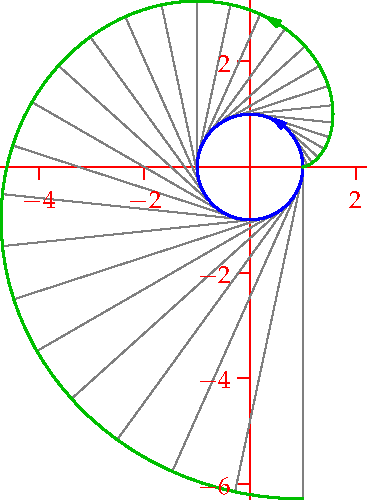
\includegraphics[scale=0.8]{radii-invcirc2}}
				&
				\href{http://math.uci.edu/~ndonalds/math162a/radii-invcat.html}{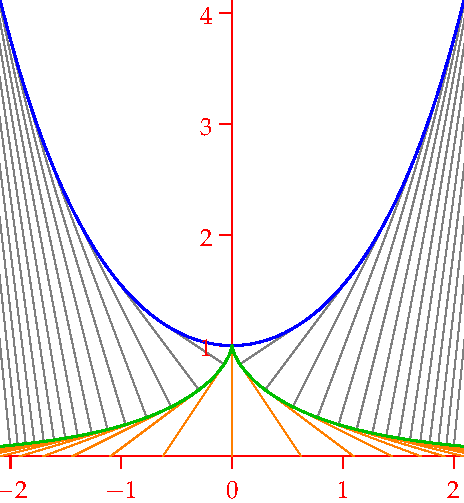
\includegraphics[scale=0.8]{radii-invcat2}}
				\\
				\textcolor{blue}{Circle} and \textcolor{Green}{involute (spiral)}
				&
				\textcolor{blue}{Catenary} and \textcolor{Green}{involute (tractrix)}
			\end{tabular}
		\end{center}
	
		Another way to visualize the involute of the catenary is to imagine attaching a weight at $(0,1)$ to a long string wrapped tightly along the catenary and then releasing the weight. Similarly, imagine a string is wound tightly around the circle and then uncoiled; the result is the involute.
	\end{enumerate}
\end{examples}



\begin{thm}{}{}
	The evolute of any involute is the original curve, except where $t=0$ or $\kappa=0$.
\end{thm}

We leave the argument as an exercise. The reverse process fails, as an observation of the parabola example should convince you: remember that an involute intersects its source curve at $t=0$\ldots

\goodbreak




\begin{exercises}
	\exstart Find the center of curvature for the curve $\vx(t)=(1-t^{-1},1+t)$ at $t=1$.
	
	
	\begin{enumerate}\setcounter{enumi}{1}
	  \item Consider the ellipse $\vx(t)=\bigl(a\cos t,b\sin t\bigr)$ where $a>b>0$.
	  \begin{enumerate}
	    \item Compute the curvature of the ellipse.
	    
	    \item Show that its evolute is the \emph{\href{https://en.wikipedia.org/wiki/Astroid}{astroid}} $\ve(t)=(a^2-b^2)\stwovec{a^{-1}\cos^3t}{-b^{-1}\sin^3t}$
	    
	    \item The four-vertex theorem states that a simple closed plane curve with differentiable curvature has at least four points where $\kappa'=0$. Show that the ellipse has precisely four.
	  \end{enumerate}
	  
	  
	  \item Describe the involutes of a straight line.\par
	  (\emph{Hint: this is a trick question!})
	  
	 
		\item In Example \ref*{ex:tractrix}.\ref{ex:tractrix1} we constructed the tractrix as the involute of the catenary.
		\begin{enumerate}
		  \item Use $\sinh^{-1}\!t=\ln\bigl(t+\sqrt{1+t^2}\bigr)$ to verify that $\vx(t)$ has unit speed and thus confirm the derivation of $\vi(t)$.
		  
		  \item Compute the tangent line to the tractrix when $t>0$ and show that this line cuts the $x$-axis a distance 1 from the curve, thus justifying the \emph{traction} claim.
		  
	  	%\item Find the curvature $\kappa(t)$ of the tractrix.
	 	\end{enumerate}
	
	
		\item\label{exs:curvetaylor} Suppose that the graph of a smooth function $y=f(x)$ passes horizontally through the origin: $f(0)=0=f'(0)$. Show that its Maclaurin series is
		\[
			f(x)\approx \frac 12\kappa(0)x^2+\text{higher order terms}
		\]
		Use this to \emph{quickly} state the curvature at $x=0$ of the graph of $y=x^2(7x^2-29)$.
	
	
		\item Let $\vx(t)$ be unit speed with non-zero curvature $\kappa$ and Frenet frame $\{\vT,\vN\}$. Moreover, let $\vi(t)=\vx(t)-t\vT(t)$ be an involute and denote the speed and corresponding data for the involute $\hat v,\hat\kappa,\hat\vT,\hat\vN$. For simplicity, suppose $\kappa,t>0$.
		\begin{enumerate}
		  \item Compute the Frenet frame of $\vi(t)$ in terms of $\vT$ and $\vN$.
		  
		  \item Show that $\hat\kappa(t)=\frac 1t$.
		  
		  \item Show that the evolute of $\vi(t)$ is the original curve $\vx(t)$.
		\end{enumerate}
		
		
		\item We see how an involute of the evolute fails to recover the original curve.\par
		Let $\vx(t)$ be regular with non-zero curvature, $\kappa'(t)\neq 0$, and evolute $\ve(t)=\vx(t)+\frac 1{\kappa(t)}\vN(t)$. Since $\ve(t)$ is regular, we may assume it is parametrized by arc-length.
		\begin{enumerate}
		  \item If $\kappa'>0$, explain why $\kappa'=\kappa^2$.
		  \item Show that the natural involute of the evolute is
		  \[
				\ve(t)-t\ve'(t)=\vx(t)+\frac 1{\kappa(0)}\vN(t)
			\]
		  that is, the original curve shifted a constant distance $\frac 1{\kappa(0)}$ in its normal direction.\par
		  (\emph{Hint: the ODE in part (a) is separable})
		  \item Find the involute of the evolute of the parabola $\vx(t)=(t,t^2)$.
		\end{enumerate}	
%   
%   \item Find the curvature of the degree $n\ge 1$ polynomial $y=x^n$ at all points (find a sensible parameteriztion of the curve first). For each $n$ find the maximum value of the curvature and the location on the curve of the point of maximum curvature (it's messy\ldots).

	\end{enumerate}
\end{exercises}


% 		\item[The Isoperimetric Inequality] states that the area in the plane bounded by a simple closed curve $\vx$ of length $l$ satisfies the inequality
% 		\[4\pi A\le l^2\quad\text{with equality}\iff\vx\text{ is a circle}.\]



